\documentclass[11pt]{article}

\usepackage[margin=1in]{geometry}
\usepackage{amsmath}
\usepackage{amssymb}
\usepackage{amsthm}
\usepackage{setspace}
\usepackage{paralist}
\usepackage{graphicx}
\usepackage{subfig}
\usepackage{url}
\usepackage{algorithm}
\usepackage{algpseudocode}
\usepackage{multicol}

\author{David~Love and G\"{u}zin~Bayraksan}

\title{Phi-Divergence Constrained Ambiguous Stochastic Programs}
\date{}

% Frequently used general mathematics
\newcommand{\R}{{\mathbb{R}}}
\newcommand{\Rp}{\R^+}
\newcommand{\Z}{{\mathbb{Z}}}
\newcommand{\Zp}{\Z^+}
\newcommand{\Q}{\mathbb{Q}}
\newcommand{\N}{\mathbb{N}}

% Commands for probability
\renewcommand{\P}{\mathbb{P}}
\newcommand{\E}{\mathbb{E}}
\newcommand{\p}[1]{\P \left[ #1 \right]}
\newcommand{\e}[1]{\E \left[ #1 \right]}
\newcommand{\ee}[2]{\E_{#1} \left[ #2 \right]}

% Definitions of variables
\newcommand{\X}{X}
\newcommand{\x}{\mathbf{x}}
\newcommand{\xh}{\hat{\x}}
\newcommand{\lh}{\hat{\lambda}}
\newcommand{\mh}{\hat{\mu}}
\newcommand{\xs}{\x^*}
\newcommand{\xit}{\tilde{\mathbf{\xi}}}
\newcommand{\zt}{\tilde{z}}
\newcommand{\zs}{z^*}

% Further variables
\newcommand{\y}{\mathbf{y}}
\renewcommand{\c}{\mathbf{c}}
\newcommand{\A}{\mathbf{A}}
\renewcommand{\b}{\mathbf{b}}
\renewcommand{\k}{\mathbf{k}}
\newcommand{\D}{\mathbf{D}}
\newcommand{\B}{\mathbf{B}}
\renewcommand{\d}{\mathbf{d}}

% Epiconvergence for \plp
\newcommand{\qtrue}{q^{\text{true}}}

% Useful mathematics functions
\newcommand{\keywords}[1]{\par\noindent\enspace\ignorespaces\textbf{Keywords:} #1}
\DeclareMathOperator*{\argmin}{argmin}
\DeclareMathOperator*{\argmax}{argmax}
\theoremstyle{plain}
\newtheorem{theorem}{Theorem}
\newtheorem{lemma}[theorem]{Lemma}
\newtheorem{proposition}[theorem]{Proposition}
\newtheorem{corollary}[theorem]{Corollary}

\theoremstyle{definition}
\newtheorem{definition}[theorem]{Definition}

\theoremstyle{remark}
\newtheorem{remark}[theorem]{Remark}
\newtheorem{property}[theorem]{Property}
\newtheorem{example}[theorem]{Example}

\newcommand{\st}{\mbox{s.t.}}

% Naming shortcuts
\newcommand{\plp}{$\phi$LP-2}

\begin{document}

\maketitle

\begin{abstract}
	This paper investigates the properties of $\phi$-divergence constrained ambiguous stochastic programs.
	$\phi$-divergences (e.g., Kullback-Leibler, $\chi^2$ distance, etc.) provide a natural way to create an ambiguity set of distributions that are centered around a nominal distribution, which is often determined by collected observations. 
	We present a classification of $\phi$-divergences to elucidate their use for models with different properties and different sources of data.
	A condition of assessing the value of collecting additional data is derived and we demonstrate convergence of the $\phi$-divergence-based ambiguous program to the associated non-ambiguous stochastic program.
	A decomposition-based solution algorithm to solve the resulting model is given.
\end{abstract}

\keywords{Ambiguous stochastic programming, phi-divergences, distributionally robust optimization, data driven methods}
%Optimization under uncertainty, water resources management,  ambiguous stochastic programming, robust optimization, environmental sustainability}

\section{Introduction and Motivation}

In practice, many optimization problems can be modeled by stochastic programs minimizing the expected value of an uncertain objective function.
However, if the distribution of the uncertain parameters used in the model is incorrect, the stochastic program can give highly suboptimal results.
Such problems have led to the development of distributionally robust optimization, a modeling technique that replaces the probability distribution by a set of distributions, and optimizes the expected cost relative to the worst distribution in the uncertainty set.
One approach that has been recently proposed by \cite{bental2011robust} uses a set of distributions that have sufficiently small $\phi$-divergence from a given ``nominal'' distribution ($\phi$-divergences provide a measure of distance between two distributions). 
Of particular interest is the case when the nominal distribution is determined by observation by making it an empirical distribution.
In this paper, we adapt the $\phi$-divergence method to the setting of a two-stage stochastic linear program with recourse and call this the two-stage $\phi$-divergence constrained ambiguous stochastic linear program with recourse (\plp).

Using $\phi$-divergences to model ambiguous probability distributions is an attractive data-driven approach because it uses the data directly---only those data points or scenarios of interest are used in the calculations.
These scenarios can come from direct observation, results of simulation, or from expert opinion that the decision maker would especially like to be robust against.
Because the \plp\ depends only on these scenarios, the size of the problem is polynomial in the sample size, making the \plp\ computationally tractable.
Furthermore, many $\phi$-divergences are commonly used in statistics (e.g, the $\chi^2$ distance) and provide a natural way of modeling problems under uncertainty. 

\subsection{Related Literature}

%\plp\ is an ambiguous stochastic program that is modeled on a two-stage minimax problem.
Stochastic programs with uncertain objective functions have long been studied by applying the minimax approach to an expected cost; see, e.g., \cite{zackova1966minimax,dupacova_87}. \cite{shapiro2002minimax} and \cite{shapiro2004class} developed methods for converting stochastic minimax problems into equivalent stochastic programs with a certain distribution.

In recent years, there has been a growing interest in distributionally robust methods.
Erdo{\u{g}}an and Iyengar \cite{erdogan2006ambiguous} study chance-constrained stochastic programs where the set of distributions considered is determined by the Prohorov metric.
Calafiore and Campi \cite{calafiore2005uncertain} develop a data-driven method for generating feasible solutions to chance constrained problems, and later Calafiore and El Ghaoui \cite{calafiore2006distributionally} develop a method for converting distributionally robust chance constraints into second-order cone constraints.
Jiang and Guan \\cite{jiang2012data} develop an exact approach to solving data-driven chance constrained programs.
Pflug and Wozabal \cite{pflug2007ambiguity} develop a data-driven method for solving a portfolio selection problem using the Kantorovich distance to define the set of distributions.
Delage and Ye \cite{delage2010distributionally} provide methods for modeling uncertain distributions of a specific form (e.g., Gaussian, exponential, etc.) or using moment-based constraints.

Three recent papers by Wang, Glynn and Ye \cite{wang2010likelihood}, Calafiori \cite{calafiore2007ambiguous}, and Hu and Hong \cite{hukullback} provide similar studies using a specific $\phi$-divergence, described in Section \ref{sec:phi_divergences}, that is defined by the Kullback-Leibler divergence.
Both \cite{wang2010likelihood} and \cite{hukullback} produce dual problems similar to that presented in \cite{bental2011robust} and used here.
Hu and Hong \cite{hukullback} differs from this work and the others by considering a continuous distributions, but doesn't relate the nominal distribution to observational data.
Additionally, \cite{klabjan2013robust} uses the $\chi^2$ distance, another $\phi$-divergence, to define an uncertain demand distribution for a stochastic lot-sizing problem using historical data.
Our work unites these previous papers and provides insight into conditions where each $\phi$-divergence should be used and the behavior of the optimization problem as more data is gathered.

\subsection{Contributions}

The contributions of this paper are as follows. 
\begin{itemize}
	\item One of the open problems identified by \cite{bental2011robust} was to study the performance of different $\phi$-divergences.
		Given that there are many $\phi$-divergences, a decision maker is left with the question of how each divergence behaves for his/her problem and which one to choose.
		We provide a novel classification of $\phi$-divergences dictated by the types of distributions that can be admitted to the set of distributions. 
		This allows us to provide insight into which class of $\phi$-divergence is most useful to which type of model.
		We note that this classification is a general feature of $\phi$-divergences and applies to a broader class of $\phi$-divergence constrained problems than the ones presented in this paper. 
		
	\item In a data-driven setting, several important questions arise.
		What happens as we add one more data?
		Will our solution change, and if so, will the overall cost decrease?
		Can we determine sampling from which scenarios result in a better (lower-cost) solution?
		Can we characterize the behavior of the problem as we add more data?
		In this paper, we provide answers to these questions.
		First, we provide a simple condition to determine if sampling from a particular scenario will rule out the current worst-case distribution, which can be generalized beyond the two-stage setting.
		Second, we show that \plp\ converges to the stochastic program with the (unknown) true distribution.
		
	\item Stochastic programs often become quite large, which raises questions of computational tractability.
		We help to answer this problem by providing a modified Bender's decomposition that can be used to solve the \plp\ efficiently by solving only linear programs. 

	\item Finally, we provide some interesting examples of $\phi$-divergences that result in commonly used risk models and illustrate our results numerically. 
\end{itemize}

\subsection{Organization}

The rest of the paper is organized as follows.
Section \ref{sec:phi_divergences} introduces the $\phi$-divergence and presents some useful properties.
Section \ref{sec:plp2} presents the derivation of $\phi$-divergence model for a two-stage stochastic program with recourse.
Section \ref{sec:classification} presents a classification of $\phi$-divergences with some examples;
Sections \ref{sec:properties} describes the data-driven properties of \plp; 
Section \ref{sec:soln_algorithm} presents a decomposition method for solving the \plp\ model; and in Section \ref{sec:comp_results} we present numerical illustrations of our results. 
%some of the properties of the \plp\ model.
We end in Section \ref{sec:concl} with conclusions and future work.
All proofs are provided in the Appendix.

%%%%%%%%%%%%%%%%%%%%%%%%%%%%%%%%%%%%%%%%%%%%%%%%%%%%%%%%%%%%%%%%%%%%%%%%%%%%%%%%
\section{Introduction to $\phi$-Divergences}
\label{sec:phi_divergences}

In this section we define the concept of a $\phi$-divergence, and describe some of the properties that will be used through the remainder of the paper.
Pardo \cite{pardo2005statistical} provides a good overview of much of the known properties of $\phi$-divergences.
Many results in this section can be also found in Ben-Tal et.\ al.\ \cite{bental2011robust}.

$\phi$-divergences are used in statistics to measure the ``distance'' between two distributions. 
In the discrete case, $\phi$-divergences can be used generally to measure the distance between two non-negative vectors $p = (p_1, \dots, p_n)^T$ and $q = (q_1, \dots, q_n)^T$, and specifically when $p$ and $q$ are probability vectors; i.e., satisfying $\sum_{\omega=1}^n p_\omega = \sum_{\omega=1}^n q_\omega = 1$.
The $\phi$-divergence is defined by
\[
	I_\phi(p,q) = \sum_{\omega=1}^n q_\omega \phi\left(\frac{p_\omega}{q_\omega}\right),
\]
where $\phi(t)$, called the $\phi$-divergence function, is a convex function on $t \geq 0$ such that $\phi(1) = 0$, and with the additional interpretations that $0 \phi(a/0) = a \lim_{t \rightarrow \infty} \frac{\phi(t)}{t}$, and $0 \phi(0/0) = 0$.
If both $p$ and $q$ are probability vectors, as we assume throughout this paper, we can additionally assume without loss of generality that $\phi(t) \geq 0$.
The function $\phi(t)$ can be modified as $\psi(t) = \phi(t) + c(t-1)$ with an appropriately chosen constant $c$ such that $\psi(t) \geq 0$ for all $t$, and $I_\psi(p,q) = I_\phi(p,q)$ for all probability vectors $p,q$.
If $\phi(t)$ is differentiable at $t = 1$ this can be done by selecting $c = -\phi'(1)$.
%; see, e.g., the Likelihood divergence and Burg entropy in Table~\ref{tb:phi_definitions}.

$\phi$-divergences are not, in general, metrics.
For example, most $\phi$-divergences do not satisfy the triangle inequality and many are not symmetric in the sense that $I_\phi(p,q) \neq I_\phi(q,p)$.
One exception is the Variation distance, which is equivalent to the $L^1$-distance between the vectors.

A $\phi$-divergence has an adjoint, defined by
\begin{equation} \label{eq:adjoint}
	\tilde{\phi}(t) = t \phi\left(\frac{1}{t}\right),
\end{equation}
which satisfies all criteria for a $\phi$-divergence \cite{bental1991certainty}, and has the property that $I_{\tilde{\phi}}(p,q) = I_\phi(q,p)$.
Divergences that are symmetric with respect to the input vectors are known as self-adjoint.

The problem formulation involves use of the conjugate $\phi^* : \R \rightarrow \R \cup \{\infty\}$, defined as
\begin{equation} \label{eq:conjugate}
	\phi^*(s) = \sup_{t \geq 0} \{st - \phi(t)\}.
\end{equation}
The conjugate $\phi^*$ is a nondecreasing convex function and may be undefined above some upper bound $\bar{s}$.

Table \ref{tb:phi_definitions} lists some common examples of $\phi$-divergences, along with their adjoints and conjugates.
For all divergences, $\phi(t) = \infty$ for $t < 0$, and the value of the conjugate is listed only in its domain; i.e., $\{s : \phi^*(s) < \infty\}$.
Most of these common divergences are widely used in statistics and information theory.
In Section \ref{ssec:special_phi}, we present other $\phi$-divergences that assign a distance of either $0$ or $\infty$, which result in commonly used risk models.
Table \ref{tb:phi_definitions} also lists a divergence, labeled ``Likelihood,'' that is somewhat different from the others.
The Likelihood divergence is equivalent to the Burg entropy when comparing probability vectors, but does not satisfy the normalizing condition $\phi(t) \geq 0$.
This divergence is included because Wang et al.\ \cite{wang2010likelihood} use it to formulate a distributionally robust newsvendor problem so that the ambiguity set of distributions have a sufficiently high empirical likelihood. 
They refer to this as the Likelihood Robust Optimization. 
We also note that \cite{calafiore2007ambiguous}, \cite{hukullback}, and \cite{wang2010likelihood} all use a different naming convention than the one given here, referring to the Likelihood divergence or Burg entropy as the ``Kullback-Leibler (KL) divergence''---reversing the order of the arguments $p$ and $q$ relative to the notation presented here.
In this paper, $q$ denotes the nominal distribution. 

\begin{table}
	\centering
	\begin{tabular}{lccccc}
		\hline \\
		Divergence                        & $\phi(t)$          & $\tilde{\phi}(t)$               & $\phi(t), t \geq 0$   & $I_\phi(p,q)$     & $\phi^*(s)$ \\
		\hline
		Kullback-Leibler                 & $\phi_{kl}$        & $\phi_b$                        & $t\log t - t + 1$     & $\sum p_\omega \log\left(\frac{p_\omega}{q_\omega}\right)$ & $e^s - 1$ \\
		Burg Entropy                      & $\phi_b$           & $\phi_{kl}$                     & $-\log t + t - 1$     & $\sum q_\omega \log\left(\frac{q_\omega}{p_\omega}\right)$ & $-\log(1-s),\ s < 1$  \\
		J-Divergence                      & $\phi_j$           & $\phi_j$                        & $(t-1)\log t$         & $\sum (p_\omega - q_\omega) \log\left(\frac{p_\omega}{q_\omega}\right)$ & No closed form \\
		Likelihood                        & $\phi_l$           & $t\log t $                      & $-\log t$             & $\sum q_\omega \log\left(\frac{q_\omega}{p_\omega}\right)$ & $-\log(-s) - 1,\ s < 0$ \\
		$\chi^2$-Distance                 & $\phi_{\chi^2}$    & $\phi_{m\chi^2}$                & $\frac{1}{t} (t-1)^2$ & $\sum \frac{(p_\omega-q_\omega)^2}{p_\omega}$              & $2 - 2\sqrt{1-s},\ s < 1$  \\
		Modified $\chi^2$-Dist.           & $\phi_{m\chi^2}$   & $\phi_{\chi^2}$                 & $(t-1)^2$             & $\sum \frac{(p_\omega - q_\omega)^2}{q_\omega}$            & $\begin{cases} -1 & s < -2 \\ s + \frac{s^2}{4} & s \geq -2 \end{cases}$ \\
% 		$\chi$-div,  $\theta > 1$ & $\phi_\chi^\theta$ & $t^{1-\theta}\phi_\chi^\theta$ & $|t-1|^\theta$         & $\sum q_\omega |1-\frac{p_\omega}{q_\omega}|^\theta$       & $\begin{cases} -1 & s \leq -\theta \\ s + (\theta-1)\left(\frac{|s|}{\theta}\right)^\frac{\theta}{\theta-1}  & s \geq -\theta \end{cases}$ \\
		Variation Distance                & $\phi_v$           & $\phi_v$                        & $|t-1|$               & $\sum |p_\omega - q_\omega|$                               & $\begin{cases} -1 & s \leq -1 \\ s & -1 \leq s \leq 1 \end{cases}$ \\
		Hellinger Distance                & $\phi_h$           & $\phi_h$                        & $(\sqrt{t} - 1)^2$    & $\sum (\sqrt{p_\omega} - \sqrt{q_\omega})^2$               & $\frac{s}{1-s},\ s < 1$ \\
	\hline
	\end{tabular}
	\caption{
		Definitions of some common $\phi$-divergences, along with their adjoints $\tilde{\phi}(t)$ and conjugates $\phi^*(s)$
	}
	\label{tb:phi_definitions}
\end{table}

%%%%%%%%%%%%%%%%%%%%%%%%%%%%%%%%%%%%%%%%%%%%%%%%%%%%%%%%%%%%%%%%%%%%%%%%%%%%%%%%
\section{$\phi$-Divergence Constrained Ambiguous Stochastic Program}
\label{sec:plp2}

In this section we provide primal and dual formulations and basic properties of two-stage ambiguous stochastic linear programs constructed via $\phi$-divergences.

%%%%%%%%%%%%%%%%%%%%%%%%%%%%%%%%%%%%%%%%%%%%%%%%%%%%%%%%%%%%%%%%%
\subsection{Formulation}
\label{ssec:form}

We begin with a two-stage stochastic linear program with recourse (SLP-2).
Let $\x$ be a vector of first-stage decision variables with cost vector $\c$, constraint matrix $\A$ and right-hand side $\b$.
We assume a finite distribution given by $q_\omega$ with scenarios indexed by $\omega = 1, \dots, n$.
The SLP-2 is
\begin{align}
	\min_\x \ & \left\{ \c\x + \sum_{\omega=1}^n q_\omega h_\omega(\x) : \A\x = \b, \x \geq 0 \right\}, \label{eq:slp_first_stage}% \\
% 	\st \ & \A\x = \b \nonumber  \\
% 	&\ \ \ \x \geq 0 \nonumber
\end{align}
where
\begin{align}
	h_\omega(\x) = \min_{\y^\omega} \ & \left\{ \k^\omega \y^\omega : \D^\omega \y^\omega = \B^\omega \x + \d^\omega, \y^\omega \geq 0 \right\}. \label{eq:slp_second_stage}
\end{align}
We assume relatively complete recourse; i.e., the second-stage problems $h_\omega(\x)$ are feasible for every feasible solution $\x$ of the first-stage problem; and that the second-stage problems $h_\omega(\x)$ are dual feasible for every feasible solution $\x$ of the first-stage problem.
For convenience, we denote $X = \{\x : \A\x = \b, \x \geq 0\}$.

The SLP-2 formulation assumes that the distribution $\{q_\omega\}_{\omega=1}^n$ is known.
However, in many applications the distribution is itself unknown.
One technique to deal with this is to replace the known distribution with an {\it ambiguity set} of distributions; i.e., a set of distributions that is believed to contain the true distribution.
In this paper, we construct the ambiguity set by considering all distributions whose $\phi$-divergence from the nominal distribution $q$ is sufficiently small.
Throughout portions of this paper, we focus on a data-driven setting and assume that $q$ is generated from observations, where scenario $\omega$ has been observed $N_\omega$ times, with $N = \sum_{\omega=1}^n N_\omega$ total observations, although $q$ can be obtained in other ways.
In SLP-2, this data-driven setting would correspond to the probability of scenario $\omega$ to be $q_\omega = \frac{N_\omega}{N}$.

By replacing the specific distribution in SLP-2 with a set of distributions sufficiently close to the nominal distribution with respect to $\phi$-divergence, we create the \plp\ model.
In the \plp, the objective function is minimized with respect to the worst-case distribution selected from the ambiguity set of distributions.
The resulting minimax formulation of \plp\ is
\begin{equation}
	\min_{\x \in X} \max_{p \in \mathcal{P}} \left\{ \c\x + \sum_{\omega=1}^{n} p_\omega h_\omega(\x) \right\}, \label{eq:plp_primal}
\end{equation}
where the ambiguity set is
\begin{align}
	\mathcal{P} = & \left\{ \sum_{\omega = 1}^{n} q_\omega \phi\left(\frac{p_\omega}{q_\omega}\right) \leq \rho, \right. \label{eq:plp_primal_divergence} \\
	& \ \sum_{\omega=1}^{n} p_\omega = 1, \label{eq:plp_primal_probability} \\
	& \ \left. p_\omega \geq 0,\ \forall \omega \right\}. \label{eq:nonneg}
\end{align}
We refer to (\ref{eq:plp_primal_divergence}) as the $\phi$-divergence constraint and (\ref{eq:plp_primal_probability}) and (\ref{eq:nonneg}) simply ensure a probability measure.
We discus how to determine $\rho$ in (\ref{eq:plp_primal_divergence}) in Section \ref{ssec:robust_level}.

Taking the dual of the inner maximization problem, with dual variables $\lambda$ and $\mu$, of constraints (\ref{eq:plp_primal_divergence}) and (\ref{eq:plp_primal_probability}), respectively, and combining the two minimizations gives \plp\ in dual form
\begin{align}
	\min_{\x,\lambda,\mu} \ & \c\x + \mu + \rho \lambda + \lambda \sum_{\omega=1}^{n} q_\omega \phi^*\left(\frac{h_\omega(\x) - \mu}{\lambda}\right) \label{eq:plp_two_stage} \\
	\st \ & \x \in X \nonumber \\
	& \frac{h_\omega(\x) - \mu}{\lambda} \leq \lim_{t \rightarrow \infty} \frac{\phi(t)}{t}, \ \forall \omega \label{eq:plp_feas_constraint}\\
	& \lambda \geq 0, \nonumber
\end{align}
where $h_\omega(\x)$ and the second-stage problems are as given in (\ref{eq:slp_second_stage}), $0\phi^*(s/0)=0$ if $s\leq 0$ and  $0\phi^*(s/0)=+\infty$ if $s > 0$.
Note that some $\phi$, such as the J-Divergence, have no closed form representation of $\phi^*$, but can be expressed as the sum of other divergences---Burg Entropy and KL divergence---which allows the dual to be formed; see \cite{bental2011robust} for details.
Theorem 1 of \cite{bental2011robust} contains a derivation of the dual problem, which is reprinted as part of the proof of Proposition \ref{prop:pop}.
Note in particular that the dual formulation is accurate even for $q_\omega = 0$ for some $\omega$.
Also note that the right-hand side of (\ref{eq:plp_feas_constraint}) contains a limit.
For some $\phi$-divergences, like the KL divergence, this limit is $\infty$, in which case (\ref{eq:plp_feas_constraint}) is redundant.
However, other $\phi$-divergences, like the Hellinger distance, have a finite limit, inducing this constraint.
Throughout the paper, we use $s_\omega$ to denote
\begin{equation}
	s_\omega = \frac{h_\omega(\x) - \mu}{\lambda}. \label{eq:s_omega_definition}
\end{equation}


%%%%%%%%%%%%%%%%%%%%%%%%%%%%%%%%%%%%%%%%%%%%%%%%%%%%%%%%%%%%%%%%%
\subsection{Basic Properties}
\label{ssec:basicprop}

In this section we list some basic properties of \plp.
Most of these have already been noted earlier (e.g., by \cite{bental2011robust} and others for specific $\phi$-divergences) but we list them for completeness.
Some of these properties help with our specialized solution method and we refer to them in later sections.

\begin{property}
	\label{property:convex}
	\plp\ is a convex program.
\end{property}

\begin{property}
	\label{property:coherent_risk_measure}
	\plp\ is equivalent to minimizing a coherent risk measure.
\end{property}

Note that being a coherent risk measure implies that \plp\ is a convex problem.
The convexity of LRO was also noted in \cite{wang2010likelihood}.

\begin{property}
	\label{property:time_structure}
	\plp\ preserves the time structure of SLP-2.
\end{property}

\begin{property}
	\label{property:primal_dual_relation}
	The worst-case distribution can be calculated with the equations
	\begin{align} 
		& \frac{p_\omega}{q_\omega} \in \partial \phi^*\left(s_\omega\right) \label{eq:p_worst} \\
		& \sum_{\omega=1}^n q_\omega \phi\left(\frac{p_\omega}{q_\omega}\right) \leq \rho \nonumber \\
		& \sum_{\omega=1}^n p_\omega = 1. \nonumber
	\end{align}
\end{property}

We now discuss these properties. A coherent risk measure is defined in \cite{rockafellar2007coherent}, which shows that minimizing a coherent risk measure over a polyhedron implies that \plp\ is a convex problem.
The convexity of \plp\ was also noted in \cite{bental2011robust}.
In Section \ref{ssec:special_phi}, we present special $\phi$-divergences that result in CVaR, or a convex combination of expectation with CVaR or the worst-case scenario. 
Properties \ref{property:time_structure} and \ref{property:primal_dual_relation} help with our decomposition-based solution method described in Section \ref{sec:soln_algorithm}. 
The preservation of time structure, as can be seen in (\ref{eq:plp_two_stage}), allows us to decompose the problem and convert (sub-)derivatives of $h_\omega(\x)$ to (sub-)derivatives of $\phi^*\left(s_\omega\right)$, aiding in our decomposition-based solution method. 
The appearance of the conjugate $\phi^*(s)$ in the objective of (\ref{eq:plp_two_stage}) gives a method for retrieving the worst-case distribution from the dual problem, as detailed in Property \ref{property:primal_dual_relation}.
In many cases, the first equation in (\ref{eq:p_worst}) is sufficient to calculate $\{p_\omega\}_{\omega=1}^n$.
In addition, $\phi^*$ is often differentiable and so we have the relationship $p_\omega = q_\omega \phi^{* \prime}(s_\omega)$.
Special cases when $\lambda = 0$ or $q_\omega = 0$ for some $\omega$ are detailed in Section \ref{sec:classification}.



%%%%%%%%%%%%%%%%%%%%%%%%%%%%%%%%%%%%%%%%%%%%%%%%%%%%%%%%%%%%%%%%%
\subsection{The Level of Robustness}
\label{ssec:robust_level}

The literature on $\phi$-divergences provides some insight on choosing a reasonable asymptotic value of $\rho$ in the data-driven setting. 
When $\phi$ is twice continuously differentiable around $1$ with $\phi^{\prime \prime}(1)>0$, Theorem 3.1 of \cite{pardo2005statistical} shows that the statistic $T^\phi_N(q^N,\qtrue) = \frac{2N}{\phi''(1)} \sum_{\omega=1}^n \qtrue_\omega \phi\left(\frac{q^N_\omega}{\qtrue_\omega}\right)$ converges in distribution to a $\chi^2$-distribution with $n-1$ degrees of freedom, where $q^N$ denotes the empirical distribution ($q^N_\omega = N_\omega/N$), and $\qtrue$ denotes the underlying true distribution.
Most $\phi$-divergences in Table~\ref{tb:phi_definitions} satisfy this differentiability condition.
\cite{bental2011robust} then use this result to suggest the asymptotic value
Ben-Tal \begin{equation} \label{eq:asymptotic_rho}
	\rho = \frac{\phi''(1)}{2N} \chi^2_{n-1,1-\alpha},
\end{equation}
where $\chi^2_{n-1,1-\alpha}$ is the $1-\alpha$ percentile of a $\chi^2_{n-1}$ distribution, which produces an approximate $1-\alpha$ confidence region on the true distribution.
For corrections for small sample sizes and more details, we refer the readers to \cite{pardo2005statistical} and \cite{bental2011robust}. 

We are now ready to present the main contributions of this paper. 

%%%%%%%%%%%%%%%%%%%%%%%%%%%%%%%%%%%%%%%%%%%%%%%%%%%%%%%%%%%%%%%%%%%%%%%%%%%%%%%%
\section{A Classification of $\phi$-Divergences}
\label{sec:classification}

Given that there are many $\phi$-divergences to choose from, it is important to study how $\phi$-divergences act within an ambiguous (or, distributionally robust) stochastic optimization model. 
We present a classification of $\phi$-divergences into four types, resulting from an examination of the limiting behavior of $\phi(t)$ as $t \rightarrow 0$ and $t \rightarrow \infty$.
Different classifications may be suitable to different problem types and desired qualities in the ambiguous model---we discuss modeling considerations with respect to our classification in Section \ref{ssec:modeling}.
We also provide some special $\phi$-divergences that result in common risk models used in the literature and discuss their behavior with respect to our classification in Section \ref{ssec:special_phi}.

%%%%%%%%%%%%%%%%%%%%%%%%%%%%%%%%%%%%%%%%%%%%%%%%%%%%%%%%%%%%%%%
\subsection{Suppressing and Popping of Scenarios}
\label{ssec:suppressandpop}

As motivation for our classification, consider a self-adjoint $\phi$-divergence, which satisfies the relation
\begin{equation} \label{eq:self_adjoint_classification}
	\frac{\phi(t)}{t} = \phi\left(\frac{1}{t}\right),
\end{equation}
and consider $t \rightarrow \infty$.
If both sides of (\ref{eq:self_adjoint_classification}) are finite in the limit, then we see a correspondence between the boundedness of $\phi(t)$ for $t < 1$ and linear growth of $\phi(t)$ for $t > 1$.
On the other hand, infinite limits of (\ref{eq:self_adjoint_classification}) indicate a correspondence between superlinear growth of $\phi(t)$ for $t > 1$ and unboundedness of $\phi(t)$ for $t < 1$.

Recall the definition of the ambiguity set, in particular, the $\phi$-divergence constraint (\ref{eq:plp_primal_divergence}). 
In the \plp, $\phi$ has arguments given by ratios of probabilities, $\tfrac{p_\omega}{q_\omega}$ and the limits $t \rightarrow 0$ and $t \rightarrow \infty$ correspond to the cases when $p_\omega = 0$ and $q_\omega = 0$, respectively.
Consider each of these limiting cases:
\begin{itemize}
	\item {\sc Case 1:} $q_\omega > 0$ but $p_\omega = 0$.
		We call this the ``{\bf Suppress}'' behavior because a scenario with a positive probability in the nominal distribution can take zero probability in the ambiguous problem. In this case we need to examine $\lim_{t \searrow 0} \phi(t)$:
	\begin{itemize}
		\item If $\lim_{t \searrow 0} \phi(t) = \infty$, the ambiguity region will never contain distributions with $p_\omega = 0$ but $q_\omega > 0$.
		\item On the other hand, if $\lim_{t \searrow 0} \phi(t) < \infty$, the ambiguity region could contain such a distribution, provided $q_\omega$ is sufficiently small or $\rho$ is sufficiently large.
			We say that such a $\phi$-divergence can \emph{suppress} scenario $\omega$.
	\end{itemize}
	\item {\sc Case 2:} $q_\omega = 0$ but $p_\omega > 0$.
		We call this the ``{\bf Pop}'' behavior because a scenario with zero probability in the nominal distribution can have a positive probability (or, pop) in the ambiguous problem. In this case, we need to examine $\lim_{t \nearrow 0} \frac{\phi(t)}{t}$:
	\begin{itemize}
		\item If $\lim_{t \nearrow 0} \frac{\phi(t)}{t} = \infty$, the ambiguity region can never contain distributions with $p_\omega > 0$ but $q_\omega = 0$.
		\item On the other hand, if $\lim_{t \nearrow 0} \frac{\phi(t)}{t} < \infty$, the ambiguity region will admit sufficiently small $p_\omega$.
			We say that these $\phi$-divergences can \emph{pop} scenario $\omega$.
	\end{itemize}
	\item {\sc Case 3:} $p_\omega = 0$ but $q_\omega = 0$.
		Such a situation has no contribution to the divergence, since $0 \phi\left(\tfrac{0}{0}\right) = 0$.
\end{itemize}

\noindent These two limiting cases describing suppressing and popping behavior in $\phi$-divergences create four distinct categories.
Examples of divergences in each category are given in Table \ref{tb:phi_categories}.
Note that $\phi$ can suppress scenarios if and only if its adjoint $\tilde{\phi}$ can pop scenarios, and vice versa.
This means that self-adjoint $\phi$-divergences are either capable of both popping and suppressing scenarios or capable of neither.

\begin{table}
	\centering
	\begin{tabular}{l|p{.33\textwidth}p{.33\textwidth}}
		 & Can Suppress Scenarios & Cannot Suppress Scenarios \\
		 \hline
		 Can Pop Scenarios %
			& \parbox{.33\textwidth}{Hellinger Distance (2),\\Variation Distance (1)} %
			& \parbox{.33\textwidth}{Burg Entropy,\\$\chi^2$-Distance} \smallskip \\
		 Cannot Pop Scenarios %
			& \parbox{.33\textwidth}{Kullback-Leibler Divergence (2),\\Modified $\chi^2$-Distance (1)} %
			& \parbox{.33\textwidth}{J-Divergence}
	\end{tabular}
	\caption{
		Examples of $\phi$-divergences fitting into each category.
		The number in parentheses under the ``Can Suppress Scenarios'' column denotes the subcategory detailed in Section \ref{ssec:suppress}.
	}
	\label{tb:phi_categories}
\end{table}

%%%%%%%%%%%%%%%%%%%%%%%%%%%%%%%%%%%%%%%%%%%%%%%%%%%%%%%%%%%%%%%
\subsection{Modeling Considerations When Choosing a Divergence}
\label{ssec:modeling}

We offer the following suggestions for choosing an appropriate $\phi$-divergence classification for the data available.
First, consider whether to choose a distribution that can suppress scenarios.
If the problem scenarios come from high-quality observed data, one may wish to avoid divergences that can suppress scenarios.
However, if the data is poorly sampled or comes from opinion rather than observation or simulation, the option of suppressing scenarios may result in a solution with better robustness properties.

Next, consider whether to choose a distribution that allows for popping scenarios.
If the problem scenarios come strictly from observation, with little theoretical understanding of the problem, we suggest choosing a divergence that cannot pop scenarios.
However, if the problem scenarios come from a mix of observed/simulated data and expert opinion about scenarios of interest, then divergences that can pop present an interesting modeling choice.
This allows for including interesting but unobserved scenarios, allowing the mathematical program to assign an appropriate probability to them.

%%%%%%%%%%%%%%%%%%%%%%%%%%%%%%%%%%%%%%%%%%%%%%%%%%%%%%%%%%%%%%%
\subsection{Additional Details about Divergences that can Suppress}
\label{ssec:suppress}

Recall the primal-dual variable relation, which specifies $\frac{p_\omega}{q_\omega} = \partial \phi^*(s_\omega)$, where $s_\omega=\frac{h_{\omega}(\x)-\mu}{\lambda}$. 
Note that suppression ($p_\omega = 0$, $q_\omega > 0$) can occur only when $0 \in \partial \phi^*(s_\omega)$.
For convenience, we assume $\phi^*$ is differentiable.
We can examine suppressing in more detail by looking at the behavior of $\phi(t)$ as $t \searrow 0$.
This analysis yields two subcategories within the $\phi$-divergences that can suppress scenarios---one tends to suppress scenarios one at a time and the other simultaneously. 

\begin{itemize}
	\item {\sc Subcategory 1\ ($\lim_{t \searrow 0} \phi'(t) > -\infty$).}  There are nonpositive constants $c,\underline{s}$ such that $\phi^*(s) = c$ for all $s < \underline{s}$. 
		Thus $\phi^{*\prime}(s_\omega) = 0$ when $s_\omega < \underline{s}$, suppressing all such scenarios.
		In other words, all scenarios that satisfy the relation $\frac{h_\omega(\x)-\mu}{\lambda} < \underline{s}$ are suppressed.
		As $\rho$ increases, scenarios tend to be suppressed one at a time.

	\item {\sc Subcategory 2\ ($\lim_{t \searrow 0} \phi'(t) = -\infty$).} In this case, $\phi^*(s) \searrow c$ as $s \rightarrow -\infty$ asymptotically, but never reaches the bound.
		As a result, scenarios can only be suppressed if $s_\omega = -\infty$, which can only occur if $\lambda = 0$ and $h_\omega(\x) < \mu$.
		Consequently, all solutions with $h_\omega(\x) < \mu$ have $p_\omega=0$, and we must have $\mu = \max_\omega h_\omega(\x)$ to ensure that scenarios $\omega \in \argmax h_\omega(\x)$ are given positive probability so that $p$ is a probability distribution.
		This means that all but the most expensive scenario(s) will vanish simultaneously.
		Divergences of this type can be difficult to deal with numerically when suppression occurs given the denominator of $\lambda = 0$ (see Section \ref{ssec:implement} for details).
\end{itemize}


Table \ref{tb:phi_categories} lists $\phi$-divergences that belong to these subcategories. We present the one-by-one and simultaneous suppressing behavior numerically for the Modified $\chi^2$-Distance and KL Divergence, respectively, in Section \ref{sec:comp_results}.

%%%%%%%%%%%%%%%%%%%%%%%%%%%%%%%%%%%%%%%%%%%%%%%%%%%%%%%%%%%%%%%
\subsection{Additional Details about Divergences that can Pop}
\label{ssec:pop}

Divergences that can pop a scenario have $\phi(t)$ grow linearly as $t \rightarrow \infty$, which causes the existence of an upper bound $\bar{s} = \lim_{t \rightarrow \infty} \frac{\phi(t)}{t}$ on the domain of $\phi^*(s)$.
The primal-dual variable relation specifies $\frac{p_\omega}{q_\omega} = \partial \phi^*(s_\omega)$, but the left-hand side is undefined when $q_\omega = 0$.
Intuitively, we can think of $\frac{p_\omega}{0} = \infty$ if $p_\omega > 0$, and thus popping a scenario can only occur when the right-hand side subdifferential also includes $\infty$.
This, in turn, occurs only when $s_\omega = \bar{s}$.
The next proposition makes this statement rigorous.

\begin{proposition} \label{prop:pop}
	Suppose there is a finite $\bar{s} = \lim_{t \rightarrow \infty} \frac{\phi(t)}{t}$.
	A scenario $\omega$ for which $q_\omega = 0$ can only be popped if $s_\omega = \bar{s}$.
\end{proposition}

\begin{remark}
	Because $s_\omega \leq \bar{s}$ for all $\omega$ and $s_\omega = \bar{s}$ for any popped scenarios, only the most expensive scenario could be popped.
\end{remark}

\begin{remark}
	Finding the probability of the popped scenario cannot be done by differentiating $\phi^*$ as with other scenarios, thus the probability must be calculated with $\sum_\omega p_\omega = 1$.
\end{remark}

%%%%%%%%%%%%%%%%%%%%%%%%%%%%%%%%%%%%%%%%%%%%%%%%%%%%%%%%%%%%%%%
\subsection{Some Special $\phi$-Divergences}
\label{ssec:special_phi}

The class of $\phi$-divergence constrained problems includes some interesting special cases, which we document here, followed by a discussion of their suppressing and popping behavior.

\begin{example}{(CVaR).}
	\label{ex:cvar}
	The coherent risk measure Conditional Value-at-Risk (CVaR) is well studied in financial applications.
	Minimizing
	\[
		\c\x + \text{CVaR}_\beta(h(\x)) = \c\x + \min_{\mu \in \R} \left\{ \mu + \frac{1}{1-\beta}\e{\left[h(\x)-\mu\right]^+} \right\}
	\]
	over $\x \in X$ is equivalent to the $\phi$-divergence constrained problem with
	\[
		\phi(t) = \
		\begin{cases}
			0 & 0 \leq t \leq \frac{1}{1-\beta} \\
			\infty & \text{otherwise},
		\end{cases}
	\]
	for $0 < \beta < 1$.

	We see that $\phi(0) = 0$, indicating that CVaR will suppress some scenarios.
	This appears in the definition of CVaR as the positive part in the expected value, $\e{[h(\x)-\mu]^+}$.
	Scenarios cannot be popped because the expectation is taken with respect to the nominal distribution.
\end{example}

The CVaR $\phi$-divergence is bounded above, which leads to the question of what happens when a divergence is bounded below.
\begin{example}[``Reverse'' CVaR]
	The $\phi$-divergence constrained problem with
	\[
		\phi(t) = \
		\begin{cases}
			0 & t \geq 1-\beta \\
			\infty & t < 1-\beta,
		\end{cases}
	\]
	for $0 < \beta < 1$ is equivalent to minimizing the convex combination of expectation and worst-case
	\[
		\c\x + \beta \sup_\omega h_\omega(\x) + (1-\beta)\e{h(\x)},
	\]
	over $\x \in X$, where the expectation is taken with respect to the nominal distribution $q$.
	Note that $\lim_{t \rightarrow \infty} \frac{\phi(t)}{t} = 0$, indicating that this divergence will pop scenarios.
	This behavior appears in the term $\sup_\omega h_\omega(\x)$.
	However, $\phi(0) = \infty$ indicates that scenarios will not be suppressed, which is demonstrated by the expectation term $\e{h(\x)}$, which takes into account every scenario with positive nominal probability.
\end{example}

An objective function taking a weighted sum of expected value and CVaR often comes up in practice.
The next example shows how to generate a convex combination of expectation and CVaR.

\begin{example}[Conbination CVaR and Expectation]
	\label{ex:cvar_expectation}
	The $\phi$-divergence constrained problem with
	\[
		\phi(t) = 
		\begin{cases}
			0 & 1-\alpha \leq t \leq \frac{1}{1-\beta} \\
			\infty & \text{otherwise},
		\end{cases}
	\]
	for $\alpha,\beta \in (0,1)$ is equivalent to minimizing, over $\x \in X$,
	\[
		\c\x + (1-\alpha)\e{h(\x)} + \alpha \mbox{CVaR}_{\frac{\beta}{\alpha(1-\beta)+\beta}}[h(\x)].
	\]
	This divergence will neither pop (because both the expectation and CVaR term are taken with respect to the nominal distribution) nor suppress (because the expectation term includes every scenario).
\end{example}

% \subsection{Variation-type Divergences}
% 
% The variation divergence is given by $\phi(t) = |t-1|$, which will result in piecewise-linear $\phi^*$.
% In general, $\phi$-divergences have a left-of-one range bounded by $\phi(0)$ and a right-of-one range bounded by $\lim_{t \rightarrow \infty} \frac{\phi(t)}{t}$.
% Consequently, we can restrict $\rho \leq 1$ for variation-type divergences.
% 
% \subsubsection{Right-sided Variation}
% 
% First, we can look only at the right-side of the variation, i.e., $\phi(t) = [t-1]^+$.
% This yields
% \[
% 	\phi^*(s) = 
% 	\begin{cases}
% 		[s]^+ & s \leq 1 \\
% 		\infty & s > 1.
% 	\end{cases}
% \]
% The upper bound on $s$ yields $\frac{h_\omega(x)-\mu}{\lambda} \leq 1$ or $\lambda \geq \sup_\omega h_\omega(x) - \mu$.
% Then starting from (\ref{eq:basic_optimization}),
% \begin{align*}
% 	\min \rho\lambda + \mu + \lambda \sum_\omega q_\omega \left[ \frac{h_\omega(x) - \mu}{\lambda} \right]^+ & = \min_{\lambda \geq \sup_\omega h_\omega(x) - \mu, \mu} \rho\lambda + \mu + \sum_\omega q_\omega \left[ h_\omega(x) - \mu \right]^+ \\
% 	& = \min_\mu \rho(\sup_\omega h_\omega(x) - \mu) + \mu \e{\left[h(x)-\mu\right]^+} \\
% 	& = \rho \sup_\omega h_\omega(x) + \min_\mu (1-\rho)\mu + \e{\left[h(x)-\mu\right]^+} \\
% 	& = \rho \sup_\omega h_\omega(x) + (1-\rho) \left( \min_\mu \mu + \frac{1}{1-\rho}\e{\left[h(x)-\mu\right]^+}\right) \\
% 	& = \rho \sup_\omega h_\omega(x) + (1-\rho) \mbox{CVaR}_\rho(h(x)).
% \end{align*}
% This time we get a convex combination between the supremum and CVaR.
% 
% \subsubsection{Left-sided Variation}
% 
% The results start getting much messier here.
% The left-sided variation is $\phi(t) = [1-t]^+$, which gives
% \[
% 	\phi^*(s) = 
% 	\begin{cases}
% 		-1 & s < -1 \\
% 		s & -1 \leq s \leq 0 \\
% 		\infty & s > 0.
% 	\end{cases}
% \]
% Once again, we have the condition $\mu \geq \sup_\omega h_\omega(x)$.
% The center linear portion will induce a CVaR-like behavior for $\frac{h_\omega(x)-\mu}{\lambda} \geq -1$, or $\mu - \lambda \leq h_\omega(x)$.
% However, the opposite condition behaves only as $\lambda$.
% Let $\bar{q} = \p{h_\omega(x) \geq \mu - \lambda}$, then using equation (\ref{eq:basic_optimization}),
% \begin{align*}
% 	\min_{\lambda \geq 0,\mu} \rho\lambda + \mu + \lambda \sum_\omega q_\omega \phi^*\left(\frac{h_\omega(x) - \mu}{\lambda}\right) 
% 	& = \min_{\lambda, \mu \geq \sup_\omega h_\omega(x)} \rho\lambda + \mu - \lambda(1-\bar{q}) + \sum_{\omega : h_\omega(x) \geq \mu - \lambda} q_\omega (h_\omega(x) - \mu) \\
% 	& = \min_{\lambda, \mu \geq \sup_\omega h_\omega(x)} \rho\lambda + (1-\bar{q})(\mu-\lambda) + \sum_{\omega : h_\omega(x) \geq \mu - \lambda} q_\omega h_\omega(x) \\
% 	& = \min_{\lambda, \mu \geq \sup_\omega h_\omega(x)} \rho\lambda + (1-\bar{q})(\mu-\lambda) + \bar{q} \mbox{CVaR}_{1-\bar{q}}(h(x)).
% \end{align*}
% $\mu-\lambda$, being the quantity that defines $\bar{q}$, is like $\mbox{VaR}(h(x))$.
% I don't know that having VaR in there makes any sense, though.
% I also can't think of any other way to simplify the above.

%%%%%%%%%%%%%%%%%%%%%%%%%%%%%%%%%%%%%%%%%%%%%%%%%%%%%%%%%%%%%%%%%%%%%%%%%%%%%%%%
\section{Data-Driven Considerations}
\label{sec:properties}

In this section we assume the nominal distribution $q$ is the empirical distribution ($q_\omega = \tfrac{N_\omega}{N}$) and provide insight into how the \plp\ changes as data is added: first how it might change with a single additional observation in Section \ref{ssec:value}, then as more and more data is gathered with asymptotic results in Section \ref{ssec:epiconvergence}.
This analysis must consider how $\rho$ changes as additional samples are taken; therefore, we use $\rho_N$ to emphasize the dependence on sample size in this section.
To be consistent with the known $\phi$-divergence results stated in Section \ref{ssec:robust_level}, we assume $\rho_N = \frac{\rho_0}{N}$.

\subsection{The Value of Data} \label{ssec:value}

With a data-driven formulation such as \plp, it is natural to ask how the optimal value and solution changes as more data is gathered.
In particular, %for robust formulations like \plp\ 
one might be concerned about being overly conservative in the problem formulation and thus missing the opportunity to find a better solution to the true distribution.
For \plp, this means that the initial model is likely to be more conservative in an effort to be robust, while the new information could make the model less conservative because new information removes the current worst-case distribution from the ambiguity set.  
Below, we present a simple method of determining if taking an additional sample will eliminate the old worst-case distribution and allow for better optimization; i.e., a lower-cost solution.
%We also provide a way of estimating the probability of sampling such an observation.

%\begin{proposition}
%	\label{prop:value}
\begin{theorem}
	\label{thm:value}
	An additional sample of scenario $\hat{\omega}$ will result in a decrease in the worst-case expected cost of the \plp\ if the following condition is satisfied
	\begin{equation} \label{eq:cost_decrease_cond}
		\sum_{\omega=1}^n q_\omega \phi^{*\prime}\left(\frac{N}{N+1}s^*_\omega\right) \left(\frac{N}{N+1}s^*_\omega\right) > \phi^*\left(\frac{N}{N+1}s^*_{\hat{\omega}}\right),
	\end{equation}
	where $s^*_\omega = \dfrac{h_\omega(\x^*_N) - \mu^*_N}{\lambda^*_N}$ and $(\x^*_N,\mu^*_N,\lambda^*_N)$ solve the $N$-sample problem with $q_\omega = \tfrac{N_\omega}{N}$.
\end{theorem}
%\end{proposition}

%All proofs are provided in the appendix.
We can interpret \eqref{eq:cost_decrease_cond} as follows. If an additional sample is taken from the unknown distribution and the resulting observed scenario $\hat{\omega}$ satisfies (\ref{eq:cost_decrease_cond}), then the $(N+1)$-sample problem will have a lower cost than the $N$-sample problem that was already solved.
This is equivalent to saying that an additional observation of $\hat{\omega}$ will rule out the computed worst-case distribution given by $\{p_\omega\}_{\omega=1}^{n}$ in \eqref{eq:p_worst}.

It is possible to simplify the condition in \eqref{eq:cost_decrease_cond} for some $\phi$-divergences and we detail this in the corollary below. 

%\begin{remark}
%	\label{rmk:cost_decrease_trick}
\begin{corollary}
	\label{cor:cost_decrease_trick}
	An additional sample of scenario $\hat{\omega}$ will result in a decrease in the worst-case expected cost of the \plp\ if the following condition is satisfied for:\vspace*{-0.1in}
	\begin{multicols}{2}
		\begin{description}
			\item[Burg entropy:] $\frac{p_{\hat{\omega}}}{q_{\hat{\omega}}} < \frac{N}{N+1}$, %(or, $p_{\hat{\omega}}<\frac{N_{\hat{\omega}}}{N}$)
			\item[$\chi^2$-distance:]  $\sum_\omega q_\omega \frac{q_\omega}{p_\omega} + \sqrt{\frac{N+1}{N}} < 2 \frac{p_{\hat{\omega}}}{q_{\hat{\omega}}}$,
			\item[Hellinger:] $\sum_\omega q_\omega \sqrt{\frac{p_\omega}{q_\omega}} + \sqrt{\frac{p_{\hat{\omega}}}{q_{\hat{\omega}}}} < 2 \frac{N}{N+1}$,
			\item[Modified $\chi^2$:] $2 \sum_\omega p_\omega \frac{p_\omega}{q_\omega} > \left(\frac{p_{\hat{\omega}}}{q_{\hat{\omega}}}\right)^2 + \left(\frac{N+1}{N}\right)^2$.
		\end{description}
	\end{multicols}
\end{corollary}


The simple conditions in Theorem~\ref{thm:value} and Corollary~\ref{cor:cost_decrease_trick} provide insight into different scenarios for a decision maker. 
Let $L = \left\{ \hat{\omega} : \sum_{\omega=1}^n q_\omega \phi^{*\prime}\left(\frac{N}{N+1}s^*_\omega\right) \left(\frac{N}{N+1}s^*_\omega\right) > \phi^*\left(\frac{N}{N+1}s^*_{\hat{\omega}}\right) \right\}$.
%That is, $L$ gives the set of scenarios that, if sampled one more observation, would result in a decrease in the optimal cost in \plp.  
Set $L$ divides the scenarios into two---the ones in $L$ guarantee a drop in the overall cost if sampled one more and therefore can be considered ``good'' scenarios. 
Note that scenarios not in $L$ can also result in the cost decrease. 
The numerical experiments in Section \ref{sec:comp_results} suggest that $L$ is an adequate indicator of ``good'' scenarios for our test problem. 
 

Finally, one might be interested in obtaining a lower bound on the probability that the next sample will decrease the optimal cost. 
An approximate lower bound on the probability of selecting a sample in $L$ can be found by solving
\begin{equation}
	\min_{r} \left\{ \sum_{\omega \in L} r_\omega \colon\ r \in \mathcal{P} \right\}. \label{eq:lb_probability}
\end{equation}
That is, we find the minimum probability of $L$ within the ambiguity set defining \plp\ (since we do not know the true distribution).
We solve (\ref{eq:lb_probability}) by taking its dual.


%%%%%%%%%%%%%%%%%%%%%%%%%%%%%%%%%%%%%%%%%%%%%
\subsection{Asymptotic Analysis}
\label{ssec:epiconvergence}

We now wish to show that \plp\ behaves essentially the same as the corresponding SLP-2 with the (unknown) true distribution $\qtrue$ as $N\rightarrow \infty$. 
%We now wish to show that the optimal value and solution of \plp\ converges to the optimal value and solution of the corresponding SLP-2 with the (unknown) true distribution $\qtrue$.
This requires that the sequence of nominal distributions converge to the true distribution $\qtrue$ in $L^\infty$, a situation that is satisfied by the assumed empirical distribution.
%In the proof, we assume $q^N = q^N^N$.
To emphasize the dependence of $N$ in the nominal distribution used, we prefer to use $q^N$ in this section. 

We begin by showing that the worst-case distribution obtained by solving the \plp\ converges weakly to the true distribution as $N \rightarrow \infty$.
Let $(\Xi,{\cal F},\P^\infty)$ be the probability space associated with taking infinitely many random samples from the distribution $\qtrue$.
Let $\Xi' \subset \Xi$ be a measure 1 set such that $\Vert q^N(\xi) - \qtrue \Vert_\infty \rightarrow 0$.

\begin{proposition} \label{prop:weak_conv}
	Suppose $\phi(t) \geq 0$ has a unique root at $t = 1$.
	%Let $p \neq \qtrue$.
	For all $\epsilon > 0$ and $\xi \in \Xi'$, there exists $N'$ such that $\forall N \geq N'$, $I_{\phi}(p,q^N(\xi)) \leq \frac{\rho_0}{N}$ implies $\max_\omega |p_\omega - \qtrue_\omega| \leq \epsilon$.
\end{proposition}

The requirements on $\phi$ in Proposition \ref{prop:weak_conv} are satisfied by every divergence in Table \ref{tb:phi_definitions} except Likelihood (which, however, can be rewritten as Burg Entropy).
The unique root requirement, however, is violated for the special cases introduced in Section \ref{ssec:special_phi}.
Proposition \ref{prop:weak_conv} implies that the worst-case distributions of (\ref{eq:plp_primal}) converge weakly to $\qtrue$, which is used to show the desired result below. 
%In the next theorem, we establish the proof that the optimal value and solution of \plp\ converges to that of the SLP-2 with distribution $\qtrue$ by establishing the epiconvergence of \plp\ to SLP-2.
\begin{theorem}
	\label{thm:epiconvergence}
	Assume $X$ is compact and $h_\omega(\x)$ are primal and dual feasible for every $\x \in X$.
	Then, the optimal value of \plp\ (\ref{eq:plp_two_stage}) converges to that of SLP-2 (\ref{eq:slp_first_stage}) with distribution $\qtrue$ and all limit points of the solutions of \plp\ solve SLP-2 with distribution $\qtrue$.
\end{theorem}

%%%%%%%%%%%%%%%%%%%%%%%%%%%%%%%%%%%%%%%%%%%%%%%%%%%%%%%%%%%%%%%%%%%%%%%%%%%%%%%%
\section{A Decomposition-Based Solution Method}
\label{sec:soln_algorithm}

As the model gets larger, a direct solution of \plp\ becomes computationally expensive. 
Decomposition-based methods could significantly reduce the solution time and allow larger problems to be solved efficiently. We propose a Bender's decomposition-based method for solving \plp.
The algorithm removes feasibility constraint (\ref{eq:plp_feas_constraint})  and exchanges it with a series of feasibility cuts in the first-stage problem.
The master problem is given by
\begin{align}
	\min_{\x,\lambda,\mu} \ & \c\x + \mu + \rho \lambda + \theta \label{eq:master_problem}\\
	\st \ & \x \in X,\ \ \lambda \geq 0 \nonumber  \\
	& \theta \geq T_j (\x,\mu,\lambda)^T + t_j, \ \  j \in J  \label{eq:objcut} \\
	& \mu + \bar{s}\lambda \geq M_k \x + m_k, \ \ k \in K \label{eq:feascut} 
\end{align}
where \eqref{eq:objcut} are the objective cuts, (\ref{eq:feascut}) are the feasibility cuts on constraint (\ref{eq:plp_feas_constraint}) if $\bar{s} = \lim_{t \rightarrow \infty} \frac{\phi(t)}{t} < \infty$, and $J$ and $K$ are the sets of objective and feasibility cuts, respectively.

The proposed algorithm is shown in Figure \ref{fig:algorithm}. 
The modified Bender's decomposition presented here has the following features:
\begin{inparaenum}[\itshape (i\upshape)]
	\item it solves the original linear second stage problems, rather than nonlinear subproblems, and uses them to quickly generate subgradients of the nonlinear term $\lambda \phi^*\left(\tfrac{h_\omega(\x) - \mu}{\lambda}\right)$, 
	\item exchanges the polyhedral $\phi$-divergence constraints $\tfrac{h_\omega(\x) - \mu}{\lambda} \leq \bar{s}$ for a (potentially much) smaller set of easily generated feasibility cuts, and thus
	\item  maintains linear master and subproblems.
\end{inparaenum}

\begin{figure}
	\centering
	\vspace{1pt}
		\begin{algorithmic}
			\State Initialize $z_l = -\infty, z_u = \infty$
			\State Solve master problem (\ref{eq:master_problem}) with $\theta = 0$ to generate $\x$
			\State Solve all second-stage scenario subproblems (\ref{eq:slp_second_stage}) to obtain $h_\omega(\x)$
			\State Initialize $\lambda \gets 1$ and $\mu$ so that $\frac{h_\omega(\x) - \mu}{\lambda} < \bar{s}$
			\State Generate initial objective cut
			\While{$z_u - z_l \geq \texttt{TOL}\min\{|z_u|,|z_l|\}$}
				\State Solve master problem (\ref{eq:master_problem}), get $\x$,$\lambda$,$\mu$,$\theta_M$
				\State Solve subproblems (\ref{eq:slp_second_stage}) to obtain  $h_\omega(\x)$
				\State $\theta_{\text{true}} \gets \sum_{\omega=1}^n q_\omega h_\omega(\x,\lambda,\mu)$
				\If{$\frac{h_\omega(\x) - \mu}{\lambda} > \bar{s}$}
					\State Generate feasibility cut
					\State Find $\mu$ so that $\frac{h_\omega(\x) - \mu}{\lambda} < \bar{s}$
				\Else
					\State $z_l \gets$ master optimal cost $\c\x + \mu + \bar{N}\lambda + \theta_{\text{true}}$
				\EndIf
				\State Generate objective cut
				\If{$\c\x + \mu + \bar{N}\lambda + \theta_{\text{true}} < z_u$}
					\State $z_u \gets \c\x + \mu + \bar{N}\lambda + \theta_{\text{true}}$
					\State $\x_\text{best} \gets \x, \lambda_\text{best} \gets \lambda, \mu_\text{best} \gets \mu$
					\State $p_\omega \gets \phi^{*\prime}(\tfrac{h_\omega(\x) - \mu}{\lambda})$ for $\omega = 1, \dots, n$
				\EndIf
			\EndWhile
		\end{algorithmic}
	\caption{Decomposition algorithm for solving \plp}
	\label{fig:algorithm}
\end{figure}

\subsection{Objective Cuts}

Let $(\xh,\mh, \lh)$ be the candidate solution from the master problem (\ref{eq:master_problem}), $\hat{s}_\omega = \frac{h(\xh)-\mu}{\lh}$, and $h^\dagger_\omega(s_\omega) = \lambda \phi^*\left(\frac{h_\omega(\x) - \mu}{\lambda}\right)$ be the nonlinear portion of the objective function, which will be used to generate the objective cuts.
An objective cut can be computed by solving the SLP-2 subproblems $h_\omega(\xh)$ to obtain the optimal dual solutions $\pi^{*,\omega}$ to each second-stage problem. Using these to compute the partial (sub)derivatives of the \plp\ subproblems
% \begin{align*}
% 	\dfrac{\partial h^\dagger_\omega(\hat{s}_\omega)}{\partial \x} & = \phi^{*\prime}(\hat{s}_\omega) \pi^{*,\omega}B^\omega, &
% 	\dfrac{\partial h^\dagger_\omega(\hat{s}_\omega)}{\partial \mu} & = -\phi^{*\prime}(\hat{s}_\omega), &
% 	\dfrac{\partial h^\dagger_\omega(\hat{s}_\omega)}{\partial \lambda} & = \phi^*(\hat{s}_\omega) - \phi^{*\prime}(\hat{s}_\omega)\hat{s}_\omega.
% \end{align*}
% The cuts are then given by
\begin{align*}
	T_j^\omega & = 
	\left( \begin{array}{ccc}
		\phi^{*\prime}(\hat{s}_\omega) \pi^{*,\omega}B^\omega, 
			 & -\phi^{*\prime}(\hat{s}_\omega), 
			 & \phi^*(\hat{s}_\omega) - \phi^{*\prime}(\hat{s}_\omega) \hat{s}_\omega
	\end{array} \right), \\
	t_j^\omega & = \lh \phi^{*\prime}(\hat{s}_\omega)\left[\hat{s}_\omega - \frac{\pi^{*,\omega}B^\omega\xh - \mh}{\lh}\right].
\end{align*}
For the single-cut master problem proposed, $T_j = \sum_\omega q_\omega T_j^\omega$ and $t_j = \sum_\omega q_\omega t_j^\omega$ and multi-cut versions are also possible. 

\subsection{Feasibility Cuts}
After the subproblems $h_\omega(\xh)$ are solved, it may be the case that $\hat{s}_\omega < \bar{s}$ for some $\omega$, rendering $\mh$ and $\lh$ infeasible.
This is corrected using the feasibility problem
\begin{align*}
	U_\omega(\x,\mu,\lambda) = \min_{y^\omega \geq 0, z \geq 0} \ & z \\
	\st \ & z + \bar{s}\lambda + \mu - q^\omega y^\omega \geq 0 \\
	& D^\omega y^\omega = d^\omega + B^\omega x,
\end{align*}
which is solved by $z = h_\omega(x) - \bar{s}\lambda - \mu$.
The subdifferentials can be easily found as $\frac{\partial z^*}{\partial \x} = \pi^{*,\omega} B^\omega$, $\frac{\partial z^*}{\partial \mu} = -1$, and $\frac{\partial z^*}{\partial \lambda} = -\bar{s}$.
Then for infeasible candidate solution $(\xh,\lh,\mh)$ we get the inequality
\begin{align*}
	U_\omega(\x,\mu,\lambda) \geq \pi^{*,\omega}B^\omega(\x-\xh) - (\mu -\mh) - \bar{s}(\lambda - \lh) + (h_\omega(\xh) - \mh - \bar{s}\lh),
\end{align*}
and setting $U_\omega(\x,\mu,\lambda) = 0$ to find a feasible solution gives the feasibility cut
\[
	\mu + \bar{s} \lambda \geq \pi^{*,\omega}B^\omega \x + (h_\omega(\xh) - \pi^{*,\omega}B^\omega\xh).
\]

% Once the feasibility cut is generated, we may need to find a feasible (and reasonable) value of $\mu$ to generate an objective cut, or to initialize the next iteration of the master problem.
% This can be done quickly by minimizing the objective function of (\ref{eq:plp_det_equiv}) with respect to $\mu$ while keeping $\xh$ and $\lh$ constant, which is equivalent to minimizing $\mu - \sum_\omega N_\omega \lh \log(\mu - h_\omega(\xh))$.
% We do this by solving the equation $\sum_\omega \frac{N_\omega \lh}{\mu - h_\omega(\xh)} = 1$ with Newton's method.

\subsection{Computational Enhancements}

In order to enhance the performance of the above decomposition algorithm, we included an $L^\infty$-norm trust region which is scaled up (by a factor of $3$) or down (by a factor of $\tfrac{1}{4}$) when the trust region inhibits finding the optimal solution or when the polyhedral lower approximation is far from the second-stage expected cost, respectively.
The trust region is an implementation of Algorithm 4.1 in \cite{nocedal1999numerical}.

\subsection{Implementation Notes on Different $\phi$}
\label{ssec:implement}

First, note that when (\ref{eq:plp_feas_constraint}) is not present, there is no need to use feasibility cuts. Let's now look at implementation issues with respect to suppression and popping. 

Divergences that can suppress in Subcategory 2 (see \S \ref{ssec:suppress}) can be computationally difficult to work with because $\lambda = 0$ could occur.
Floating point finite tolerance can alleviate this somewhat for the KL divergence, for which $\phi^*(s) = e^s$, because $e^{-800} = 0$ to machine precision.
We recommend forcing $\lambda$ to be nonzero and checking optimality condition at $\lambda = 0$ separately.

Divergences that can pop require a check for any $s_\omega = \bar{s}$.
The probability of a popped scenario can be determined by enforcing $\sum_\omega p_\omega = 1$ after determining the probability of the other scenarios.

For divergences that cannot pop, it can be useful to add a computational upper bound on $s$, $\bar{s}_\text{comp}$.
Such an upper bound can be computed easily by bounding the ratio $\frac{p_\omega}{q_\omega} \leq \frac{1}{\min_\omega q_\omega}$.
The computational upper bound can then be selected so that $\phi^{*\prime}(\bar{s}_\text{comp}) \geq \frac{1}{\min_\omega q_\omega}$.
Note, however, that an artificial upper bound will induce artificial popping behavior if the nominal distribution contains impossible scenarios.
This technique is especially useful for the KL divergence because $e^s$ overflows on double-precision machines for $s \geq 710$.



%%%%%%%%%%%%%%%%%%%%%%%%%%%%%%%%%%%%%%%%%%%%%%%%%%%%%%%%%%%%%%%%%%%%%%%%%%%%%%%%
\section{Numerical Illustration} \label{sec:comp_results}

To illustrate the techniques discussed in this paper, we applied the decomposition method from Section \ref{sec:soln_algorithm} to a small electricity generation problem.
On this problem, we demonstrate the popping and suppressing behavior described in Section \ref{sec:classification} for several $\phi$-divergences and show how the worst-case cost decrease condition (\ref{eq:cost_decrease_cond}) compares to the actual cost decrease when an additional sample of each scenario is taken.

We modified an SLP-2 test problem, denoted APL1P, which is a power expansion problem with 5 independent random variables and 1280 realizations \cite{infanger1992monte}.
To clearly demonstrate how the worst-case distribution changes with $\rho$ and especially to demonstrate suppressing and popping behavior, we took 6 unique samples from APL1P to form the \plp. 
We denote the resulting problem as $\phi$APL1P. 
The first-stage determines the capacity to be built for two generators and the generators are operated under uncertain demands and availability of the generators in the second stage.

In this problem, the second scenario (displayed in green in Figures \ref{fig:suppress} and \ref{fig:pop}) is the most costly, thus the only candidate for popping. %if its nominal probability vanishes.
Furthermore, the second scenario will eventually have unit probability in suppressing divergences.
%All scenarios are assumed to have a single observation, unless popping behavior is being demonstrated.

\subsection{Numerical Results}
\label{ssec:numerical_results}

Table \ref{tb:numerical_results} shows a few select results for the $\phi$APL1P using different $\phi$-divergences.  
Behavior is shown assuming one observation per scenario for divergences above the line, and with the most costly scenario unobserved below the line to demonstrate popping.
The value of $\rho$ is chosen in accordance with an asymptotic $95\%$ confidence region in (\ref{eq:asymptotic_rho}).
For the popping example, while $n=6$ is the same, $N$ is one less, resulting in a different $\rho$. 

All divergences put the highest probability in the most costly scenario. 
Notice that, at this level of robustness, the Modified $\chi^2$-Distance has suppressed three scenarios, while the KL divergence has not yet suppressed any.
In the next section, as $\rho$ increases, the KL divergence will suppress all but the most costly scenario simultaneously. 
The total costs are similar except for the Burg entropy with popping, which is slightly lower.


\begin{table}
	\centering
	\begin{tabular}{cc|c|cccccc}
		$\phi$ & $\rho$ & Cost & \multicolumn{6}{c}{Worst-Case Distribution} \\
		\hline
		$\phi_{m\chi^2}$ &  1.845  & 30735 & 0.1353 & 0.6354 & 0.2293 & 0      & 0      & 0 \\
		$\phi_{kl}$      &  0.9225 & 30921 & 0.1050 & 0.7208 & 0.1507 & 0.0052 & 0.0108 & 0.0075 \\
		$\phi_b$         &  0.9225 & 30714 & 0.0636 & 0.7751 & 0.0768 & 0.0253 & 0.0308 & 0.0285 \\
		\hline
		$\phi_b$         &  1.107  & 29775 & 0.1065 & 0.6273 & 0.1311 & 0.0402 & 0.0494 & 0.0455
	\end{tabular}
	\caption{
		Numerical results of $\phi$APL1P for various divergences.
	}
	\label{tb:numerical_results}
\end{table}

\subsection{Illustrations of Popping and Suppressing}
\label{ssec:numerical_pop_suppress}

%DAVID: I'm removing this first paragraph as it is repeating stuff.

%Section \ref{sec:classification} discussed a method of classifying $\phi$-divergences into four types based on two criteria: whether a $\phi$-divergences allows distributions that suppress certain scenarios (i.e., allows $p_\omega = 0$ while $q_\omega > 0$); and whether a $\phi$-divergence allows distributions that pop a scenario that is impossible in the nominal distribution (i.e., allows $p_\omega > 0$ while $q_\omega = 0$).
%In this section we present computational results demonstrating the suppressing and popping behavior of different divergences.
%The categorization of several $\phi$-divergences can be found in Table \ref{tb:phi_categories}.

We begin with an examination of two divergences that can suppress scenarios.
Figure \ref{fig:suppress} shows how the worst-case distribution changes with $\rho$ for both the Modified $\chi^2$-Distance (left) and the KL divergence (right).
As shown in Section \ref{ssec:suppress}, the Modified $\chi^2$-Distance suppresses scenarios one at a time, starting with the least expensive; while the KL divergence will suppress all (simultaneously) but the most costly scenario.

An example of a $\phi$-divergence that can pop, the Burg entropy, is given in Figure \ref{fig:pop}.
The left plot in Figure \ref{fig:pop} demonstrates the worst-case distribution assuming that all scenarios have a single observation.
The right plot shows the worst-case distribution when all scenarios but the most costly have a single observation, which is unobserved.
Notice, in particular, that the probability of the most costly scenario becomes small as $\rho$ decreases.
Other divergences that can pop but not suppress look qualitatively similar.

\begin{figure}
	\includegraphics*[width=.45\textwidth]{images/mchi2}%
	\includegraphics*[width=.45\textwidth]{images/kl}%
	\caption{
		Examples of distributions that can suppress: Modified $\chi^2$ distance (left; one-at-a-time suppression) and KL Divergence (right; simultaneous suppression).
	}
	\label{fig:suppress}
\end{figure}


\begin{figure}
	\includegraphics*[width=.42\textwidth]{images/burg}%
	\includegraphics*[width=.42\textwidth]{images/burg_zero}%
	\caption{
		Example of a distribution that can pop---the Burg entropy: 
		all scenarios have a single observation (left); 
		 the most costly scenario having no observation (right).
	}
	\label{fig:pop}
\end{figure}

\subsection{Illustration of Value of Data}
\label{ssec:numerical_value_of_data}

A comparison of the worst-case expected cost decrease condition (\ref{eq:cost_decrease_cond}) with the actual decrease in expected cost resulting from an additional observation is shown in Figure \ref{fig:value} for the Modified $\chi^2$-Distance (left) and the Burg Entropy (right).
The solid lines indicate regions where (\ref{eq:cost_decrease_cond}) is satisfied and dotted regions indicate that (\ref{eq:cost_decrease_cond}) is not satisfied.
Note that (\ref{eq:cost_decrease_cond}) is a sufficient but not necessary condition.
Both plots were generated using the reformulations to (\ref{eq:cost_decrease_cond}) provided in Corollary \ref{cor:cost_decrease_trick}.
The most costly scenario, shown in green in all plots, is not visible in Figure \ref{fig:value} because an additional observation will increase the worst-case expected cost.
Condition (\ref{eq:cost_decrease_cond}) was never satisfied for this scenario.

\begin{figure}
	\includegraphics*[width=.45\textwidth]{images/mchi2_decrease_condition}%
	\includegraphics*[width=.45\textwidth]{images/burg_decrease_condition}%
	\caption{
		Decrease in the worst-case expected cost from an additional observation  for Modified $\chi^2$-Distance (left) and Burg Entropy (right).
		Solid lines indicate when (\ref{eq:cost_decrease_cond}) is satisfied, while dotted lines show when an additional observation decrease the worst-case expected cost although (\ref{eq:cost_decrease_cond}) is not satisfied.
	}
	\label{fig:value}
\end{figure}

\subsection{Generalized Network Water Model} 
\label{ssec:network_model}

We applied \plp\ to a multi-period generalized network flow model of Colorado River water allocation in Tucson, defined by a set of nodes and directed arcs $(N,\: A)$.
The nodes represent available water supply from the Colorado River, water treatment plants, reservoirs, and water demand sites.
The arcs represent the conveyance system (pipes, etc.) that carry water between the nodes. 
Water can be stored in between time periods in reservoirs to meet future demands. 
The model aims to find the minimal cost water flows considering energy, treatment, storage, and transportation costs over the planning period. 
Generalized network water allocation models have been used to find water allocations and delivery reliabilities and to assess values of different water use operations; see, e.g., \cite{draper_etal_03}. 

Water flows on arc $(i,j) \in A$ during time period $t = 1, \dots, P$ are represented by decisions $x_{ijt}$.
Each arc $(i,j) \in A$ and time period $t$ has a unit cost $c_{ijt}^x$, loss coefficient $0 \leq a_{ijt} \leq 1$ to account for evaporation, leakage from the pipes, etc., and bounds on the flow $l_{ijt}^x \leq x_{ijt} \leq u_{ijt}^x$.
Each node $j \in N$ has a supply/demand for time period $t$, $b_{jt}$.
Nodes representing reservoirs are able to store water between time periods.
Stored water available at node $j$ at the beginning of time period $t$ is $s_{jt}$, with associated cost $c_{jt}^s$ and bounds $l_{jt}^s \leq s_{jt} \leq u_{jt}^s$.
Finally, water released into the environment from node $j$ in period $t$ is given by $r_{jt}$, with bounds $l_{jt}^r \leq r_{jt} \leq u_{jt}^r$.
The deterministic model is a multi-period generalized network flow model of the form
\begin{align*}
	\min_{x,s,r} \ & \sum_{(i,j) \in A} \sum_{t=1}^P c_{ijt}^x x_{ijt} + \sum_{j \in N} \sum_{t=1}^P c_{jt}^s s_{jt}\\
	\st \ & \sum_{i \in N} x_{jit} + s_{j,t+1} + r_{jt} = \sum_{i \in N} a_{ijt} x_{ijt} + s_{jt} + b_{jt}, \ \ \forall j,t \\
	& l_{ijt}^x \leq x_{ijt} \leq u_{ijt}^x,\ \ \ \forall i,j,t \\
	& l_{jt}^s \leq s_{jt} \leq u_{sjt}^s, \ \ \ \forall j,t \\
	& l_{jt}^r \leq r_{jt} \leq u_{sjt}^r, \ \ \ \forall j,t.
\end{align*}

The model is converted to a two-stage stochastic model with $P_1$ periods in the first stage and $P-P_1$ stages in the second stage.
We assume that the supplies and demands are uncertain, as well as the bounds on the decision variables.
\begin{align}
	\min_{(x,s,r) \in L^1} \ & \sum_{(i,j) \in A} \sum_{t=1}^{P_1} c_{ijt}^x x_{ijt} + \sum_{j \in N} \sum_{t=1}^{P_1} c_{jt}^s s_{jt} + \sum_{\omega=1}^n p_\omega h_\omega(s) \label{eq:gen_network_two_stage} \\
	\st \ & \sum_{i \in N} x_{jit} + s_{j,t+1} + r_{jt} = \sum_{i \in N} a_{ijt} x_{ijt} + s_{jt} + b_{jt},\ \ \ \ \forall j, 1 \leq t \leq P_1, \notag
\end{align}
where the second stage problems
\begin{align}
	h_\omega(s) = \min_{(x,s,r) \in L^2_\omega} \ & \sum_{(i,j) \in A} \sum_{t=P_1+1}^{P} c_{ijt}^x x_{ijt} + \sum_{j \in N} \sum_{t=P_1+1}^{P} c_{jt}^s s_{jt} \label{eq:gen_network_second_stage} \\
	\st \ & \sum_{i \in N} x_{jit} + s_{j,t+1} + r_{jt} = \sum_{i \in N} a_{ijt} x_{ijt} + s_{jt} + b_{jt}^\omega, \ \ \ \ \forall j, P_1+1 \leq t \leq P, \notag
\end{align}
and $L^1$ and $L^2_\omega$ represent the feasible regions defined by the lower and upper variable bounds.

% In the rest of the paper, we simplify the notation for the first-stage (\ref{eq:gen_network_two_stage}) and second-stage (\ref{eq:gen_network_second_stage}) problems as follows.
% In the first stage, decision variables $\{x_{ijt}\}$, $\{s_{jt}\}$ and $\{r_{jt}\}$ become the vector $\x$, costs $\{c_{ijt}^x\}$ and $\{c_{jt}^s\}$ are written as the row vector $\c$, the supply/demand parameters $b_{jt}$ become the vector $\b$ and the constraint matrix is written as $A$.
% In the second stage, we denote the decisions as $\y^\omega$, the costs as $\k^\omega$, the supply/demands as $\d^\omega$, and the constraint matrices multiplying $\y^\omega$ and $\x$ as $D^\omega$ and $B^\omega$, respectively.

% Using the generalized network model (\ref{eq:gen_network_two_stage}) of Colorado River water allocation in the southeastern portion of Tucson, we created a likelihood robust water allocation problem of the form \plp.
% The southeastern portion of Tucson is a newly developing area and is expected to grow considerably. 
% The \plp\ water allocation model would help authorities with future water plans in this area while being robust to uncertainties in water supplies and demands.

The model has a total of $P = 41$ time periods, representing years 2010--2050. 
%, with projections coming from studies WISP \cite{??} and TAZ \cite{??}.
% We use $P_1 = 10$ time periods for the first stage, and four second-stage scenarios are constructed from high (WISP) and low (TAZ) population estimates along with high and low estimates for the amount of water available for use.
For each time period, the network has 62 nodes representing demand for potable and nonpotable (reclaimed) water, pumps, water treatment plants, and the available water supply from the Colorado River.
The network in each time period has 102 arcs, representing the pipe network carrying the water between the nodes physically and connecting the network to the five reservoirs that connect the time stages in the model.
We use $P_1 = 10$ time periods for the first stage.
Uncertainty in the second stage takes the form of uncertain population (thus, demand for water) and supply of water.
There are a total of 4 scenarios considered in this test instance: (i) high population, high supply, (ii) high population, low supply, (iii) low population, high supply, and (iv) low population, low supply.
Each scenario is assumed to have five observations.
The high population scenarios are more costly as the system needs to meet demand or pay for unmet demand.
The low population scenarios, on the other hand, are not as costly. 
% The supply variability seems to have a nominal effect.
We applied the decomposition-based solution algorithm presented in Section \ref{sec:soln_algorithm} to solve this model.% and selected tolerances $\texttt{TOL} = 10^{-5}$ and $\texttt{TOL2} = 10^{-3}$ for our computational experiments.

\subsection{Computational Results}

Figure \ref{fig:worst_case} shows how the worst-case distribution changes with $\gamma'$.
When $\gamma'$ is close to $1$, we use the maximum likelihood distribution, which has equal $\tfrac{1}{4}$ probabilities on each of the four scenarios.
As $\gamma'$ is decreased, the ambiguity set increases, and the worst-case distribution used by \plp\ changes.
It gives higher than $\tfrac{1}{4}$ probability to the two high-population scenarios and lower than $\tfrac{1}{4}$ probability to the two low-population scenarios, making the solution more robust to costly scenarios.
Note that the scenarios fall into two similar pairs because the cost of each scenario depends strongly on the projected demand but only weakly on the projected supply of Colorado River water.
A closer look at the optimal solutions reveals that as $\gamma'$ is decreased, or as robustness is increased, the solution uses more and more reclaimed water (treated wastewater that is reused for nonpotable purposes such as irrigation) in an effort to meet demands in a least-costly way.

\begin{figure}
	\centering
	\subfloat[][Worst-case distribution]{
		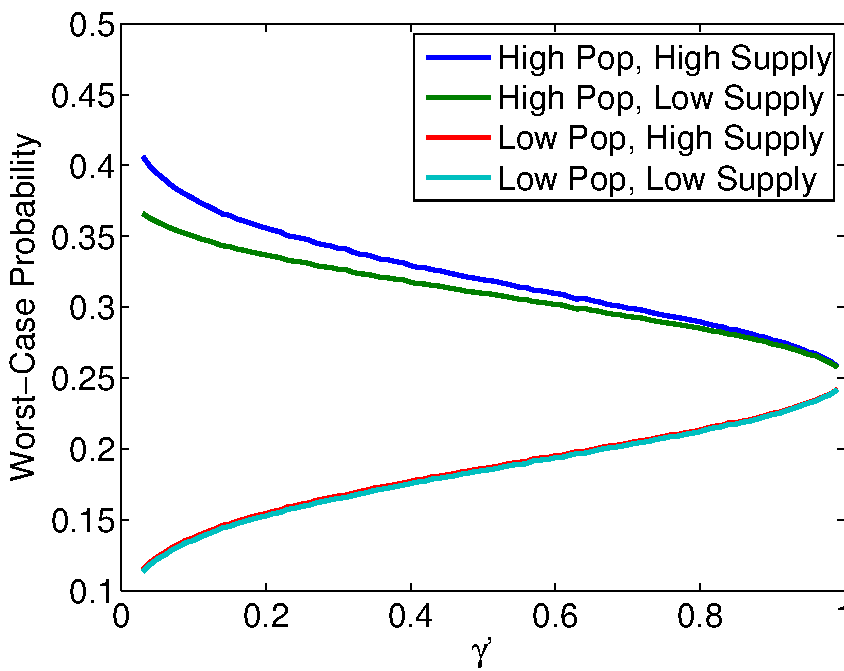
\includegraphics[width=.45\textwidth]{images/worst_case_probability}
		\label{fig:worst_case}
	}%
	\subfloat[][Probability of cost decrease]{
		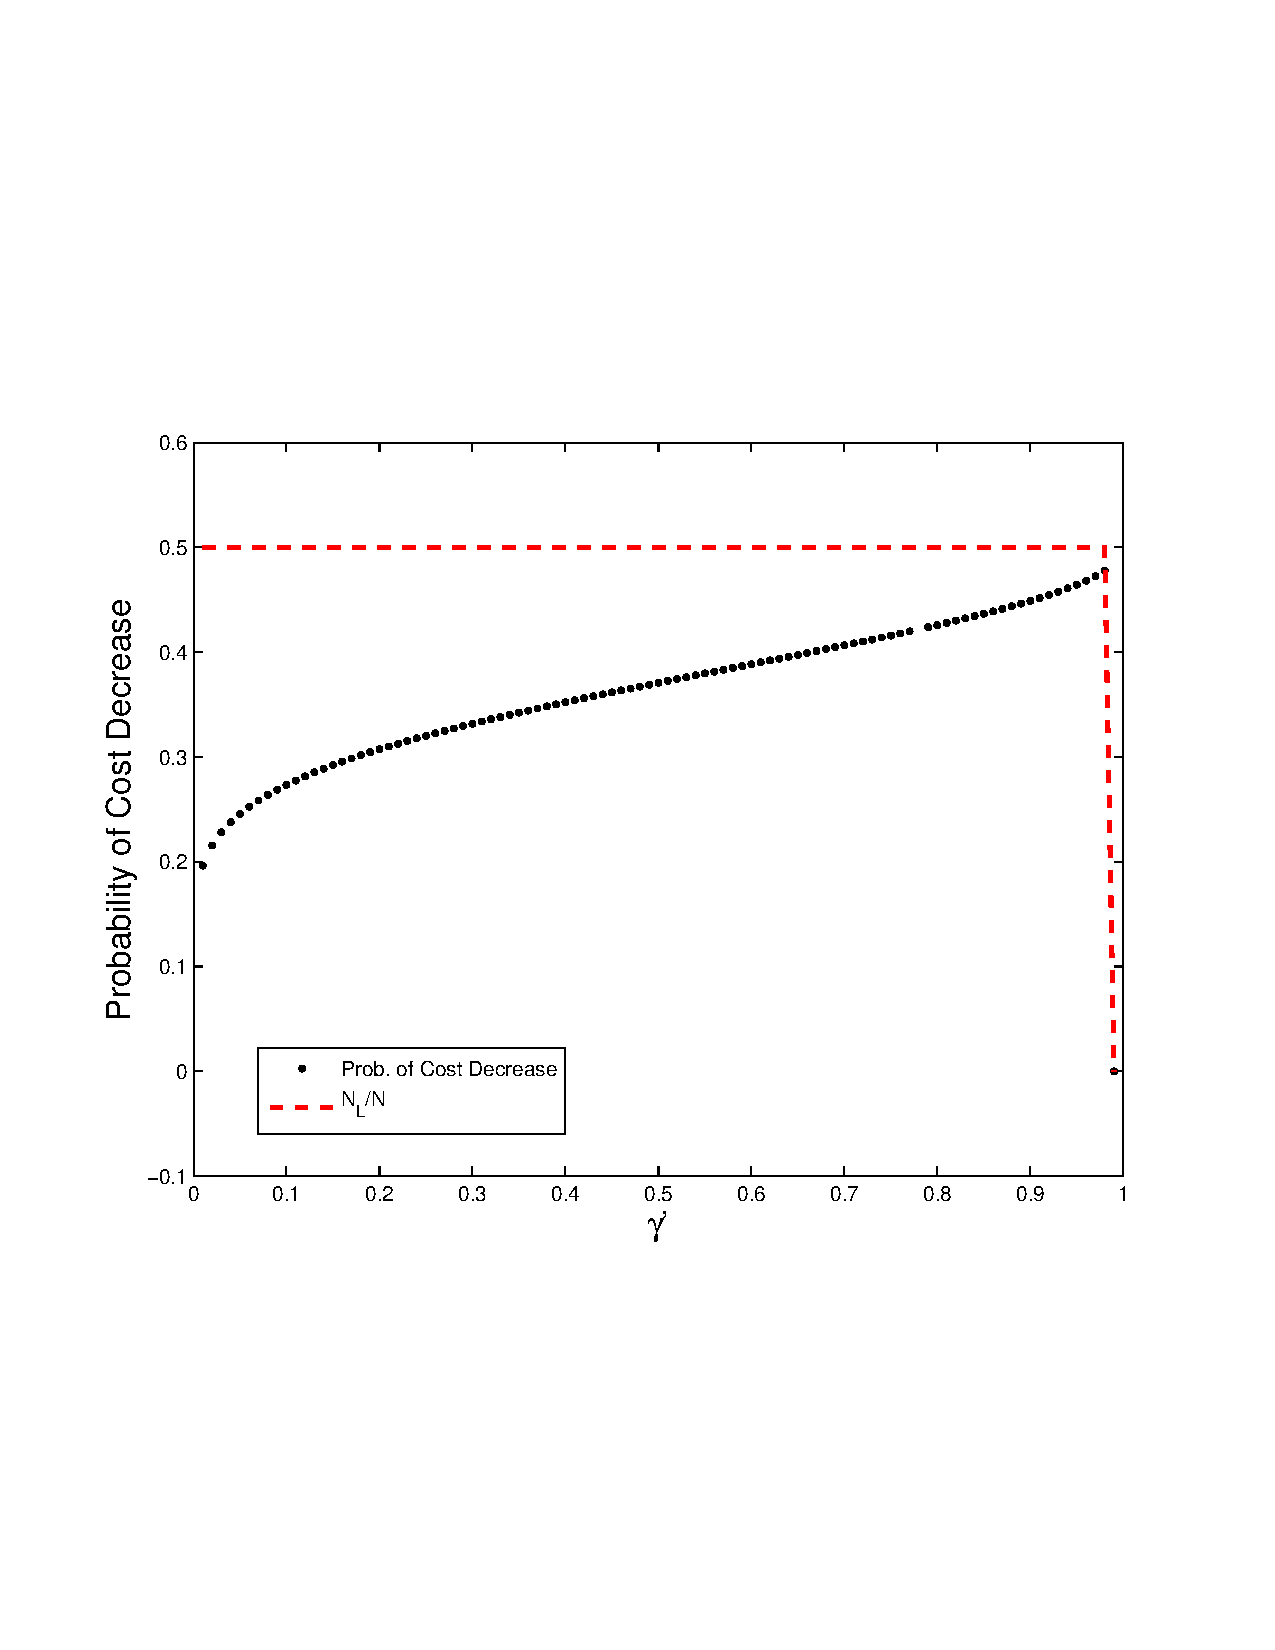
\includegraphics[width=.45\textwidth]{images/water_prob_decrease}
		\label{fig:water_prob_decrease}
	}
	\caption{%
		(a) Worst-case distribution for the likelihood robust water allocation problem.
		(b) Probability that an additional sample causes a decrease in worst-case expected cost for the likelihood robust water allocation problem.
		The red line shows the upper bound probability $\tfrac{N_L}{N}$.
	}
\end{figure}

%\subsection{Value of Data}

The results of the water model were then analyzed with the value of data techniques from Section \ref{ssec:value}.
Figure \ref{fig:water_prob_decrease} shows the estimated probability that an additional sample will remove the worst-case distribution from the likelihood region, resulting in a lower-cost solution. %, analogous the results of Figure \ref{fig:prob_cost_decrease_gp}.
The dashed line in Figure \ref{fig:water_prob_decrease} depicts the computed values of $\frac{N_L}{N}$, which provide an upper bound on the estimated probabilities. 
Because the low-population scenarios have lower costs, an additional sample of either low-population scenario will result in a lower expected cost.
This is what we see through most of the computed values of $\gamma'$, with $\frac{N_L}{N} = 0.5$, indicating that the sufficient condition (\ref{eq:cost_decrease_cond}) was satisfied for both low-population scenarios.
For extremely large values of $\gamma'$---above $0.97$---we see the ratio $\frac{N_L}{N}$ quickly drops to zero.
This occurs because (\ref{eq:cost_decrease_cond}) only compares scenario probabilities in the empirical ($N_\omega / N$) and worst-case ($p_\omega$) distributions and does not use the computed cost of the scenarios.
As $\gamma'$ increases and the ambiguity set shrinks, the worst-case probabilities become so close the empirical probabilities that (\ref{eq:cost_decrease_cond}) can no longer be satisfied, resulting in $\frac{N_L}{N}$ decreasing to zero.
% 
% \begin{figure}
% 	\centering
% 	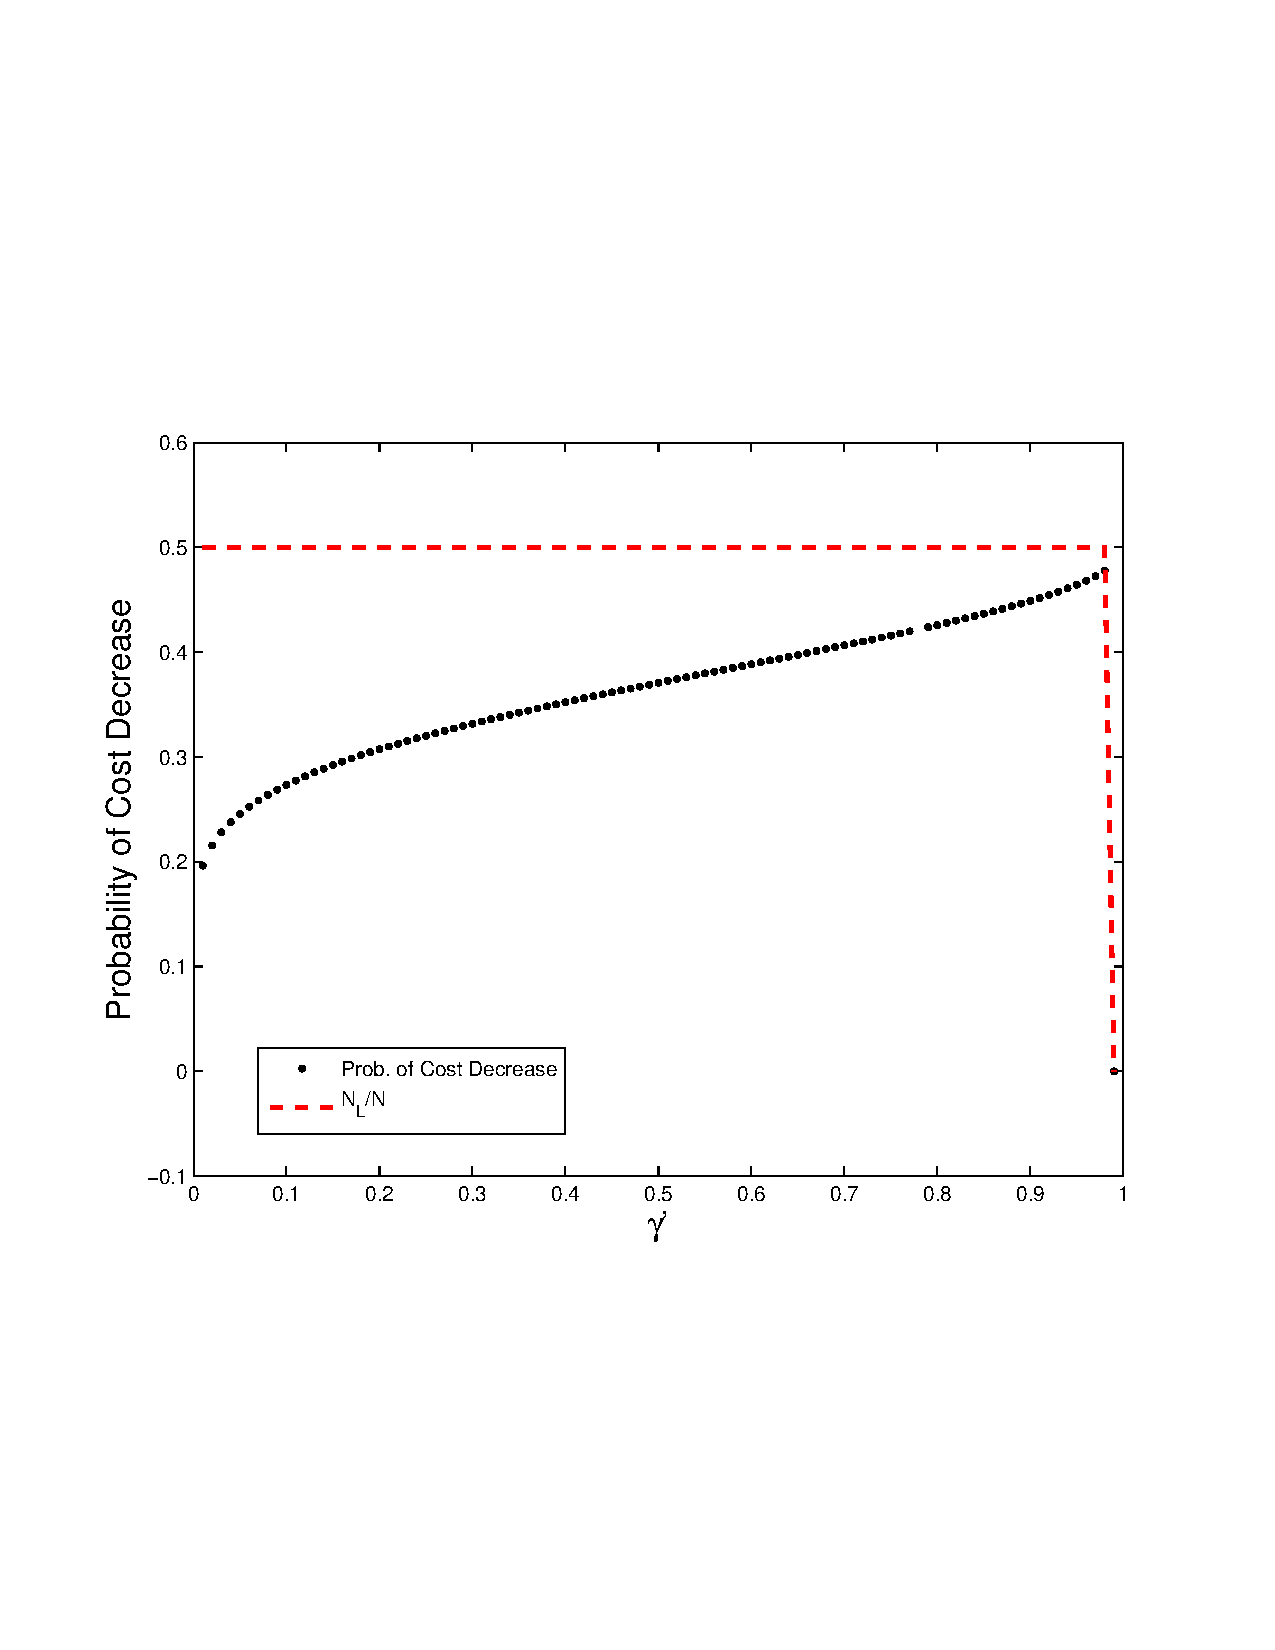
\includegraphics[width=.5\textwidth]{images/water_prob_decrease}
% 	\caption{Probability that an additional sample causes a decrease in worst-case expected cost for the likelihood robust water allocation problem.  The red line shows the upper bound probability $\tfrac{N_L}{N}$.}
% 	\label{fig:water_prob_decrease}
% \end{figure}

%%%%%%%%%%%%%%%%%%%%%%%%%%%%%%%%%%%%%%%%%%%%%%%%%%%%%%%%%%%%%%%%%%%%%%%%%%%%%%%%
\section{Summary and Future Work}
\label{sec:concl}

We proposed to use $\phi$-divergences
% constrained distributionally robust optimization method of \cite{bental2011robust} for two-stage stochastic linear programs with recourse, creating a two-stage $\phi$-divergence constrained ambiguous stochastic linear program with recourse, denoted \plp.
%The \plp\ uses a $\phi$-divergence 
to define an ambiguity set of probability distributions, possibly using observed data, and optimize the worst-case expected cost with respect to this ambiguity set in a two-stage setting.
We provided a new classification of $\phi$-divergences that can be used in determining which $\phi$-divergence is most appropriate in practice for different model types and decision makers.
A computationally simple method is established to determine if an additional sample %will produce a likelihood ambiguity set that does not contain the current worst-case distribution and
will result in a lower-cost solution.
We have shown that as more data is gathered, the optimal value and solution of \plp\ converge to those of SLP-2. 
We have also provided a Bender's decomposition-based solution algorithm to solve \plp\ efficiently and used it to illustrate some of the properties of the \plp.
% on a small electricity generation problem.

There are many interesting avenues for future work. 
One is the multi-stage extensions of the work provided here. 
Ways to handle continuous distributions in the \plp\ also merits further research. 
There are other divergences, probability metrics, and statistical ways to measure the distance between two distributions. 
Generalizations of the results presented in this paper to other distance measures is another area of future research. 
Finally, it would be useful to study applications to real-world problems.


\appendix
\section{Proofs}

\noindent In this appendix, we provide proofs of all propositions, theorems, and the corollary in the order they appear in the paper. 

\begin{proof}{\sc Proof of Property \ref{property:coherent_risk_measure}}
	Rockafellar also shows that $\cal R$ is a coherent risk measure if and only if it can be written using a risk envelope \cite{rockafellar2007coherent}.
	We will show that \plp\ can be written in the form of a risk envelope in the primal form (\ref{eq:plp_primal}) with the change of variables $\tilde{p}_\omega = \frac{p_\omega}{1/n}$.
	Throughout the proof, all expectations are taken with respect to the uniform distribution.
	
	First, probability constraint (\ref{eq:plp_primal_probability}) can be written as $\e{\tilde{p}} = 1$, where $\tilde{p}$ is the random variable taking values $\tilde{p}_\omega$ with equal probability.
	Then the $\phi$-divergence constraint (\ref{eq:plp_primal_divergence}) becomes $\sum_{\omega=1}^n \frac{1}{n} \tilde{p}_\omega \frac{\phi\left(\tilde{p}_\omega/\tilde{q}_\omega\right)}{\tilde{p}_\omega/\tilde{q}_\omega} \leq \rho$, where $\tilde{q}_\omega = \frac{q_\omega}{1/n}$ and $\frac{\phi(a/0)}{a/0} = \lim_{t \rightarrow \infty} \frac{\phi(t)}{t}$.
	Combining these yields the set ${\cal Q} = \{\tilde{p} | \e{\tilde{p}} = 1, \sum_{\omega=1}^n \frac{1}{n} \tilde{p}_\omega \frac{\phi\left(\tilde{p}_\omega/\tilde{q}_\omega\right)}{\tilde{p}_\omega/\tilde{q}_\omega} \leq \rho \}$, a closed and convex risk envelope.
	Finally, we can rewrite the inner maximization of (\ref{eq:plp_primal}) as $\max_{\tilde{p} \in {\cal Q}} \e{\tilde{p} h(x)}$, where $h(x)$ is the random variables defined by $\{h_\omega(x)\}$.
	Thus we see that \plp\ is the minimum of a coherent risk measure.
\end{proof}

\begin{remark}
	The above proof can be simplified by using $\tilde{p}_\omega = \frac{p_\omega}{q_\omega}$ if $q_\omega > 0$ for all $\omega$.
	However, the case of $q_\omega = 0$ plays an important role in the classification presented in Section \ref{sec:classification}.
\end{remark}

\begin{proof}{\sc Proof of Proposition \ref{prop:pop}.}
	We present here an abridged derivation of the dual problem (\ref{eq:plp_two_stage}), which can be found in full in \cite{bental2011robust}, and additionally consider the case where $q_\omega = 0$.
	For this proof, we assume for simplicity that the first-stage cost vector $\c = 0$.	
	We begin with the Lagrangian of (\ref{eq:plp_primal}), $\mathcal{L}(p,\mu,\lambda) = \sum_{\omega=1}^n p_\omega h_\omega(\x) + \left( 1-\sum_{\omega=1}^n p_\omega \right)\mu + \left( \rho - \sum_{\omega=1}^n q_\omega \phi\left(\frac{p_\omega}{q_\omega}\right) \right)\lambda$, for which we generate the dual problem as
	\begin{align}
		 & \min_{\lambda \geq 0, \mu} \max_{p \geq 0} \sum_{\omega=1}^n p_\omega h_\omega(\x) + \left( 1-\sum_{\omega=1}^n p_\omega \right)\mu + \left( \rho - \sum_{\omega=1}^n q_\omega \phi\left(\frac{p_\omega}{q_\omega}\right) \right)\lambda \nonumber \\
		& = \min_{\lambda \geq 0, \mu} \mu + \rho\lambda + \sum_{\omega=1}^n \max_{p_\omega \geq 0} \left\{ p_\omega (h_\omega(\x) - \mu) - \lambda q_\omega \phi\left(\frac{p_\omega}{q_\omega}\right) \right\} \label{eq:pop_proof_detail_1} \\
		& =  \min_{\lambda \geq 0, \mu} \mu + \rho\lambda + \lambda \sum_{\omega=1}^n q_\omega \max_{t_\omega \geq 0} \left\{ s_\omega t_\omega - \phi(t_\omega) \right\} \label{eq:pop_proof_detail_2} \\
		& = \min_{\lambda \geq 0, \mu} \mu + \rho\lambda + \lambda \sum_{\omega=1}^n q_\omega \phi^*\left(s_\omega\right), \nonumber
	\end{align}
	where $t_\omega = \frac{p_\omega}{q_\omega}$.
	
	To account for the possibility that $q_\omega = 0$ and demonstrate popping behavior, equality (\ref{eq:pop_proof_detail_2}) must be modified slightly.
	Consider a term in the summation in (\ref{eq:pop_proof_detail_1}) for which $q_\omega = 0$:
	\begin{align}
		\max_{p_\omega \geq 0} \left\{ p_\omega (h_\omega(\x) - \mu) - \lambda q_\omega  \phi\left(\frac{p_\omega}{q_\omega}\right) \right\} & = \max_{p_\omega \geq 0} \left\{ p_\omega (h_\omega(\x) - \mu) - \lambda 0  \phi\left(\frac{p_\omega}{0}\right) \right\} \nonumber \\
		& = \max_{p_\omega \geq 0} \left\{ p_\omega \left( h_\omega(\x) - \mu - \lambda \bar{s} \right) \right\}. \label{eq:pop_proof_condition}
	\end{align}
	The behavior of (\ref{eq:pop_proof_condition}) depends on the sign of $\left( h_\omega(\x) - \mu - \lambda \bar{s}  \right)$, or equivalently, relation between $s_\omega$ and $\bar{s}$.
	There are three cases:
	\begin{description}
		\item[Case 1: $s_\omega > \bar{s}$] selects $p_\omega = \infty$, which induces the constraint $\frac{h_\omega(\x) - \mu}{\lambda} \leq \bar{s}$ for scenarios with $q_\omega = 0$.
		\item[Case 2: $s_\omega < \bar{s}$] selects $p_\omega = 0$.
		\item[Case 3: $s_\omega = \bar{s}$] places no restrictions on the value of $p_\omega$, since (\ref{eq:pop_proof_condition}) is identically zero, and hence allows for $p_\omega > 0$ (popping).\qedhere
	\end{description}
\end{proof}

\begin{proof}{\sc Proof of Example \ref{ex:cvar}}
	First, note that for a random cost $h_\omega(x)$, $\mbox{CVaR}_\beta(h(x)) = \sup_{P \in \mathcal{P}} \{\e{PH(x)}\}$, where the risk envelope is given by
	\[
		\mathcal{P} = \left\{ P \left| P \leq \frac{1}{1-\beta}, \e{P} = 1, P \geq 0 \right.\right\}.
	\]
	This risk envelope motivates the choice of $\phi(t)$.
	
	Note that this $\phi$ only admits two distance values: $0$ or $\infty$.
	Thus any choice of $\rho < \infty$ is equivalent to $\rho = 0$.
	
	The conjugate is
	\[
	\phi^*(s) = \
		\begin{cases}
			0 & s < 0 \\
			\frac{1}{1-\beta} s & s \geq 0,
		\end{cases}
	\]
	which results in the objective function given by
	\begin{align*}
		\min_{\lambda \geq 0,\mu} \mu + \rho \lambda + \lambda \sum_\omega q_\omega \phi^*\left( \frac{h_\omega(x)-\mu}{\lambda} \right) & = \min_{\lambda \geq 0, \mu} \mu + 0\lambda + \lambda \sum_\omega q_\omega \max\left\{ 0, \frac{1}{1-\beta} \frac{h_\omega(x)-\mu}{\lambda} \right\} \\
		& = \min_{\mu} \mu + \frac{1}{1-\beta} \sum_\omega q_\omega \max\left\{ 0, h_\omega(x)-\mu \right\} \\
		& = \min_{\mu} \mu + \frac{1}{1-\beta} \e{[h(x)-\mu]^+},
	\end{align*}
	which is one definition of CVaR.
\end{proof}

\begin{proof}{\sc Proof of Example \ref{ex:cvar_expectation}}
	Without loss of generality, let $\rho = 0$.
	The conjugate is
	\[
		\phi^*(s) = 
		\begin{cases}
			(1-\alpha) s & s < 0 \\
			\frac{1}{1-\beta} s & s \geq 0.
		\end{cases}
	\]
	
	This gives the problem
	\begin{align*}
		\min_{\lambda \geq 0,\mu} \mu + \rho \lambda + \lambda \sum_\omega q_\omega \phi^*\left(\frac{h_\omega(x)-\mu}{\lambda}\right) & = \min_\mu \mu + \sum_\omega q_\omega \max \left\{ (1-\alpha)(h_\omega(x)-\mu), \frac{(h_\omega(x)-\mu)}{1-\beta} \right\}.
	\end{align*}
	Now, CVaR includes a $\e{[\cdot]^+}$ term, which can be found in the maximum formula.
	Noting that $1-\alpha < 1 < \frac{1}{1-\beta}$, rewrite the maximum as
	\[
		\max \left\{ (1-\alpha)(h_\omega(x)-\mu), \frac{(h_\omega(x)-\mu)}{1-\beta} \right\} = (1-\alpha)(h_\omega(x)-\mu) + \left( \frac{1}{1-\beta} - (1-\alpha) \right) \left[ h_\omega(x)-\mu \right]^+.
	\]
	Then working with the linear term and writing in terms of expectations we get
	\[
		(1-\alpha)\e{h(x)} + \min_\mu \alpha\mu + \left( \frac{1}{1-\beta} - (1-\alpha) \right) \e{h(x)-\mu}^+
	\]
	which simplifies to
	\[
		(1-\alpha)\e{h(x)} + \alpha \min_\mu \left\{ \mu + \left(1 - \frac{\beta}{\alpha(1-\beta)+\beta}\right)^{-1} \e{h(x)-\mu}^+ \right\}
	\]
	and thus
	\[
		(1-\alpha)\e{h(x)} + \alpha \mbox{CVaR}_{\frac{\beta}{\alpha(1-\beta)+\beta}}[h(x)]. \qedhere
	\]
\end{proof}

\begin{proof}{\sc Proof of Theorem \ref{thm:value}.}
	For ease of exposition, we assume $\phi^*$ is differentiable, although the proof works without this assumption with little modification.	
	We begin this proof with the change of variables $\kappa = \frac{\lambda}{N}$, and note that $N\rho_N = \rho_0$ is constant.	
	With this change of variables, the objective function is given by
	\[
		f_N(\x,\mu,\kappa) = c\x + \mu + \rho_0 \kappa + \sum_{\omega = 1}^n N_\omega \left[ \kappa \phi^*\left(\frac{h_\omega(\x) - \mu}{N\kappa} \right) \right].
	\]
	Let $z_N = \min_{\x,\mu,\kappa} f_N(\x,\mu,\kappa)$.
	We wish to find a simple estimate of the decrease in the optimal cost, $z_N - z_{N+1}$, associated with taking an additional sample of, say, $\hat{\omega}$, looking in particular for a condition under which $z_N - z_{N+1} > 0$.	
	Let $(\x^*_N,\mu^*_N,\kappa^*_N)$ minimize $f_N$.
	Then $z_N - f_{N+1}(\x^*_N,\mu^*_N,\kappa^*_N)$ is a lower bound on the decrease in optimal cost $z_N - z_{N+1}$.
	We will find scenarios $\hat{\omega}$ such that $z_N - f_{N+1}(\x^*_N,\mu^*_N,\kappa^*_N) > 0$.

	The objective of the $N+1$ sample problem for a given $(\x,\mu,\kappa)$ is $\c\x + \mu + \rho_0 \kappa + \sum_{\omega = 1}^n N'_\omega \left[ \kappa \phi^*\left(\frac{h_\omega(\x) - \mu}{(N+1)\kappa} \right) \right]$,	where $N'_\omega$ is the number of observations of $\omega$ after $N+1$ total observations.
	Then the difference between the two optimal costs is $\kappa \sum_{\omega=1}^n \left[ N_\omega \phi^*\left(\frac{h_\omega(\x) - \mu}{N\kappa} \right) - N'_\omega \phi^*\left(\frac{h_\omega(\x) - \mu}{(N+1)\kappa} \right) \right]$, which must be positive to guarantee a drop in optimal cost.
	Let $\hat{\omega}$ be the scenario observed on the next observation, then we can rewrite the condition as
	\begin{equation} \label{eq:raw_cond}
		\kappa \sum_{\omega=1}^n N_\omega \left[ \phi^*\left(\frac{h_\omega(\x) - \mu}{N\kappa} \right) - \phi^*\left(\frac{h_\omega(\x) - \mu}{(N+1)\kappa} \right) \right] - \kappa \phi^*\left(\frac{h_{\hat{\omega}}(x) - \mu}{(N+1)\kappa}\right) > 0.
	\end{equation}

	Let $s^N_\omega = \frac{h_\omega(x) - \mu}{N\kappa}$ and $s^{N+1}_\omega = \frac{h_\omega(x) - \mu}{(N+1)\kappa}$, and note that $s^{N+1}_\omega = \tfrac{N}{N+1} s^N_\omega$.
%	Let $|\Delta s| = | s^{N+1}_\omega - s^N_\omega | = \frac{|s^{N+1}_\omega|}{N}$.
	The difference $\phi^*(s^N_\omega) - \phi^*(s^{N+1}_\omega)$ will be approximated by the derivative.
%	Note that $\phi^*(s)$ is nondecreasing because $0 \leq t = \phi^{*\prime}(s)$ for some $t$.
%	First, for $s^N_\omega > 0$, $\phi^*(s^N_\omega) - \phi^*(s^{N+1}_\omega) \geq \phi^{*\prime}(s^{N+1}_\omega) |\Delta s|$.
%	Then for $s^N_\omega < 0$, $\phi^*(s^{N+1}_\omega) - \phi^*(s^N_\omega) \leq \phi^{*\prime}(s^{N+1}_\omega) |\Delta s|$, and thus $\phi^*(s^N_\omega) - \phi^*(s^{N+1}_\omega) \geq -\phi^{*\prime}(s^{N+1}_\omega) |\Delta s|$.
%	Then both cases reduce to $\phi^*(s^N_\omega) - \phi^*(s^{N+1}_\omega) \geq \frac{1}{N} \phi^{*\prime}(s^{N+1}_\omega) s^{N+1}_\omega$.
Note that $\phi^*(s)$ is convex, so, using the gradient inequality we have $\phi^*(s^N_\omega) - \phi^*(s^{N+1}_\omega) \geq \frac{1}{N} \phi^{*\prime}(s^{N+1}_\omega) s^{N+1}_\omega$. 
	Using this, we can guarantee (\ref{eq:raw_cond}) is satisfied with the condition $\kappa \sum_{\omega=1}^n \frac{N_\omega}{N} \phi^{*\prime}(s^{N+1}_\omega) s^{N+1}_\omega - \kappa \phi^*\left(\frac{h_{\hat{\omega}}(x) - \mu}{(N+1)\kappa}\right) > 0$, or, rearranging and dividing by $\kappa > 0$,
	\begin{equation} \label{eq:main_value_derivation}
		\sum_{\omega=1}^n \frac{N_\omega}{N} \phi^{*\prime}(s^{N+1}_\omega) s^{N+1}_\omega > \phi^*(s^{N+1}_\omega).
	\end{equation}
	Finally, return to the original variables with the substitution $s^{N+1}_\omega = \frac{N}{N+1} s^*_\omega$
\end{proof}


\begin{proof}{\sc Proof of Corollary \ref{cor:cost_decrease_trick}.}
%	We use a small trick to transform condition (\ref{eq:cost_decrease_cond}) into a form that is easier to work with.
	%Recall that 
	For any real number $c$, we can define $\phi_c(t) = \phi(t) + c(t-1)$, which satisfies $I_{\phi_c}(p,q) = I_\phi(p,q)$ for probability vectors $p$ and $q$.
	This changes the conjugate as $\phi_c^*(s) = \phi^*(s-c) + c$.
	For some $\phi$, we can choose $c$ such that $\phi^{*\prime}(s)$ is separable, i.e., $\phi^{*\prime}(as) = f(a) \phi^{*\prime}(s)$ for some function $f$.
	Using this separability, we can simplify (\ref{eq:cost_decrease_cond}) for some $\phi$, after some algebra, by choosing:\vspace*{-0.15in}
	\begin{multicols}{2}
	\begin{description} 
		\item[Burg entropy:]  $c = -1$, so $\phi^{*\prime}(s) = -\frac{1}{s}$,
		\item[$\chi^2$-distance:] $c = -1$, so $\phi^{*\prime}(s) = \frac{1}{\sqrt{-s}}$,
		\item[Hellinger:]  $c = -1$ so $\phi^{*\prime}(s) = \frac{1}{s^2}$, 
		\item[Modified $\chi^2$:] $c = 2$, so
		\[
			\phi^{*\prime}(s) = \
			\begin{cases}
				\frac{1}{2} s & s \geq 0 \\
				0 & s < 0.
			\end{cases} \qedhere
		\]
	\end{description}
	\end{multicols}
\end{proof}

\begin{proof}{\sc Proof of Proposition \ref{prop:weak_conv}.}
	Let $Z = \{\omega : \qtrue_\omega = 0\}$ be the set of impossible scenarios.
	For simplicity, we assume $\epsilon$ is chosen so that $\max_{\omega \notin Z} \qtrue_\omega > \frac{\epsilon}{2}$ and drop the dependence on $\xi \in \Xi'$.	
	First, note that $\max_\omega |p_\omega - \qtrue_\omega| \leq \max_\omega |p_\omega - q^N_\omega| + \max_\omega |q^N_\omega - \qtrue_\omega|$.
	Let $N''$ be such that $\max_\omega |q^N_\omega - \qtrue_\omega| \leq \frac{\epsilon}{2}$ for all $N \geq N''$.
	To complete the proof, we will show that one can choose $N' \geq N''$ such that $\forall N \geq N'$, $\max_\omega |p_\omega - q^N_\omega| > \frac{\epsilon}{2} \Rightarrow I_\phi(p,q) > \frac{\rho_0}{N}$.
	First, bound the divergence by
	\begin{align}
		I_{\phi}(p,q^N) & = \sum_{\omega=1}^n q^N_\omega \phi\left( \frac{p_\omega}{q^N_\omega} \right) \nonumber \\
		& = \bar{s} \mathbb{I}_{\bar{s} < \infty} \sum_{\omega \in Z} p_\omega + \sum_{\omega \notin Z} q^N_\omega \phi\left( \frac{p_\omega}{q^N_\omega} \right) \nonumber \\
		& \geq \bar{s} \mathbb{I}_{\bar{s} < \infty} \sum_{\omega \in Z} p_\omega + \min_{\omega \notin Z} \{q^N_\omega\} \cdot \max_{\omega \notin Z} \left\{ \phi \left( \frac{p_\omega}{q^N_\omega} \right) \right\} \nonumber \\
		& \geq \bar{s} \mathbb{I}_{\bar{s} < \infty} \sum_{\omega \in Z} p_\omega  + \min_{\omega \notin Z} \{q^N_\omega\} \cdot \min\left\{ \phi\left(1+\frac{\epsilon}{2}\right), \phi\left(1-\frac{\epsilon}{2}\right) \right\} \label{eq:asymptotic_proof_phi_substitution} \\
		& \geq \bar{s} \mathbb{I}_{\bar{s} < \infty} \sum_{\omega \in Z} p_\omega + \min_{\omega \notin Z} \left\{ \qtrue_\omega - \frac{\epsilon}{2} \right\} \cdot \min\left\{ \phi\left(1+\frac{\epsilon}{2}\right), \phi\left(1-\frac{\epsilon}{2}\right) \right\} \nonumber,
	\end{align}
	where $\bar{s}\mathbb{I}_{\bar{s} < \infty}$ is the indicator function taking value $\bar{s}$ if $\bar{s} < \infty$ (i.e., if $\phi$ can pop scenarios---please see Section~\ref{ssec:suppressandpop} for details), and zero otherwise.	
	Inequality (\ref{eq:asymptotic_proof_phi_substitution}) is true because $\phi \left( \frac{p_\omega}{q^N_\omega} \right) \geq \min\left\{ \phi\left( \frac{q^N_\omega+\tfrac{\epsilon}{2}}{q^N_\omega} \right), \phi\left( \frac{q^N_\omega-\tfrac{\epsilon}{2}}{q^N_\omega} \right) \right\}$ for at least one $\omega$, and applying the inequalities $\frac{a+\eta}{a} \geq 1 + \eta$ and $\frac{a-\eta}{a} \leq 1-\eta$.
	
	Finally, choose $N'$ to satisfy $\bar{s} \mathbb{I}_{\bar{s} < \infty} \sum_{\omega \in Z} p_\omega + \min_{\omega \notin Z} \left\{ \qtrue_\omega - \frac{\epsilon}{2} \right\} \cdot \min\left\{ \phi\left(1+\frac{\epsilon}{2}\right), \phi\left(1-\frac{\epsilon}{2}\right) \right\} \geq \frac{\rho_0}{N'}$.
\end{proof}

\begin{proof}{\sc Proof of Theorem \ref{thm:epiconvergence}.}
	The theorem can be proven by showing the epiconvergence of the objective function of \plp\ to that of SLP-2.
	To this end, we apply Proposition \ref{prop:weak_conv} to Theorem 3.7 of \cite{dupacova1988asymptotic}, which establishes the epiconvergence of (\ref{eq:plp_primal}) under the evident conditions that the objective function (under the worst-case distribution) is continuous with respect to $\omega$ (because $\omega$ is discrete) and lower semicontinuous and locally lower Lipschitz with respect to $x$ (because \plp\ is convex).
\end{proof}


\section*{Acknowledgements}
Support provided by a Water Sustainability Program Fellowship through the Technology and Research Initiative Fund at the University of Arizona.
This work has also been partially supported by the National Science Foundation through grant CMMI-1151226.

\bibliographystyle{plain}
\bibliography{love_lro}


%\section*{Author Biographies}

%\noindent {\bf DAVID LOVE} is a graduate student in the Graduate Interdisciplinary Program in Applied Mathematics at the University of Arizona.
%His research interests include distributionally robust stochastic programming and water resources management.
%His email address is \url{dlove@math.arizona.edu} and his web page is \url{http://math.arizona.edu/~dlove}.

%\bigskip

%\noindent {\bf G\"{U}ZIN BAYRAKSAN} is an Associate Professor of Integrated Systems Engineering at the Ohio State University.
%Her research interests include Monte Carlo sampling methods for stochastic programming and applications to water resources.
%Her email address is \url{bayraksan.1@osu.edu} and her web page is \url{http://www-iwse.eng.ohio-state.edu/biosketch_GBayraksan.cfm}

\end{document}
